\documentclass[DIN, pagenumber=false, fontsize=11pt, parskip=half]{scrartcl}

\usepackage[english]{babel}
\usepackage[utf8]{inputenc}
\usepackage[T1]{fontenc}
\usepackage{textcomp}
\usepackage{amsmath} 
\usepackage{graphicx}
\usepackage{float}
\usepackage[colorlinks=true, linkcolor=blue, urlcolor=blue]{hyperref}
\usepackage{circuitikz}


% for matlab code
% Remove 'bw' option to enable colored syntax highlighting
\usepackage[framed,numbered]{mcode}

\setlength{\parindent}{0em}

% Custom headers
\setkomafont{section}{\normalfont\bfseries\Large}
\setkomafont{subsection}{\normalfont\bfseries\large}

\newcommand{\mytitle}[1]{{\noindent\Huge\textbf{#1}}}
\newcommand{\mypart}[1]{\vspace{1cm}\hrule\vspace{0.5cm}\noindent\textbf{\LARGE #1}\vspace{0.5cm}\hrule\vspace{1cm}}
\newcommand{\myproblem}[1]{\subsection*{#1}}

%===================================
\begin{document}

\noindent\textbf{GENG8030-MATLAB} \hfill \textbf{University of Windsor}\\
Winter 2026 \hfill Bob Little\\

\mytitle{\Large Course Notes \hfill \today}

\vspace{1cm}
\noindent\textbf{\large Table of Contents}
\vspace{0.5cm}

\begin{itemize}
    \item \hyperref[tut1]{Tutorial 01: An Overview of MATLAB}
    \item \hyperref[tut2]{Tutorial 02: Numeric, Cell and Structure Arrays}
    \item \hyperref[tut3]{Tutorial 03: Functions}
    \item \hyperref[tut4]{Tutorial 04: Programming with MATLAB}
    \item \hyperref[tut9]{Tutorial 09: Numerical Methods}
    \item \hyperref[tut10]{Tutorial 10: Simulink}
\end{itemize}

\vspace{0.5cm}

%===================================
% TUTORIAL 1 SECTION
%===================================
\label{tut1}
\mypart{Tutorial 01: An Overview of MATLAB}

%===================================
% KEY SUMMARY — Tutorial 1 Concepts
%===================================

\section*{Key Concepts and Common Pitfalls (Tutorial 1 Summary)}

\subsection*{1. MATLAB Arithmetic and Precedence Rules}

MATLAB follows a strict order of precedence:
\begin{itemize}
    \item Parentheses
    \item Exponentiation
    \item Multiplication and division
    \item Addition and subtraction
\end{itemize}

Incorrect placement of parentheses can completely change results.
For example:
\[
27^{1/3} \neq 27^1/3
\]

\textcolor{red}{\textbf{Pitfall:}}
Students frequently misinterpret expressions such as:
\begin{lstlisting}
16^-1/2
16^(-1/2)
\end{lstlisting}
which produce different answers due to operator precedence.

\subsection*{2. Scalar Operations vs Mathematical Notation}

MATLAB syntax must be explicit:
\begin{itemize}
    \item Multiplication requires \texttt{*}
    \item Division requires clear parentheses
\end{itemize}

Example:
\begin{lstlisting}
(3*y)/(4*x-8)   % Correct
3*y/4*x-8       % Often misinterpreted
\end{lstlisting}

\textcolor{red}{\textbf{Pitfall:}} Missing parentheses leads to unintended evaluation order.

\subsection*{3. Numerical Limits: Overflow and Underflow}

MATLAB floating-point limits can produce:
\begin{itemize}
    \item \texttt{Inf} when numbers exceed \texttt{realmax}
    \item \texttt{0} or precision loss near \texttt{realmin}
\end{itemize}

Example concept:
\begin{lstlisting}
x1 = a*b*d;    % may overflow
x2 = a*(b*d);  % safer evaluation
\end{lstlisting}

\textcolor{red}{\textbf{Pitfall:}} Intermediate calculations may overflow even if final results are valid.

\subsection*{4. Built-in Functions and Units}

Key MATLAB functions:
\begin{itemize}
    \item \texttt{log()} = natural logarithm
    \item \texttt{log10()} = base-10 logarithm
    \item Trigonometric functions use radians
\end{itemize}

\textcolor{red}{\textbf{Pitfall:}}
Confusing \texttt{log()} with base-10 logarithm is a very common mistake.

\subsection*{5. Arrays and Vectorization}

MATLAB operates efficiently on arrays:
\begin{lstlisting}
u = 0:0.1:10;
w = 5*sin(u);
\end{lstlisting}

Vectorized operations compute many values at once.

\textcolor{red}{\textbf{Pitfall:}}
Using matrix operators instead of element-wise operators:
\begin{itemize}
    \item Use element-wise operators for arrays: \verb|.*|, \verb|./|, \verb|.^|.
\end{itemize}

\subsection*{6. Plotting Basics}

Core plotting workflow:
\begin{lstlisting}
plot(x,y)
xlabel('x')
ylabel('y')
grid on
\end{lstlisting}

Important steps:
\begin{itemize}
    \item Define domain first
    \item Use consistent units
    \item Label axes clearly
\end{itemize}

\textcolor{red}{\textbf{Pitfall:}}
Forgetting element-wise operators when computing functions for plotting.

\subsection*{7. Script Files and Execution Order}

When MATLAB executes a name:
\begin{enumerate}
    \item Checks variables
    \item Checks built-in commands
    \item Searches current folder
    \item Searches path
\end{enumerate}

\textcolor{red}{\textbf{Pitfall:}}
Naming scripts the same as MATLAB functions causes execution errors.

\subsection*{8. Engineering Problem-Solving Workflow}

Recommended steps:
\begin{itemize}
    \item Define inputs and outputs clearly
    \item Verify with simple hand calculations
    \item Perform a reality check on results
\end{itemize}

\textbf{Common Mistake:}
Trusting MATLAB output without verifying physical meaning or units.

\subsection*{9. Debugging Strategy}

Typical error types:
\begin{itemize}
    \item Syntax errors (missing brackets, commas)
    \item Runtime errors (division by zero)
\end{itemize}

Recommended debugging methods:
\begin{itemize}
    \item Remove semicolons to inspect values
    \item Test simplified cases
    \item Check intermediate variables
\end{itemize}


\vspace{1cm}
\hrule
\vspace{0.5cm}

\section*{Tutorial Problems}

\myproblem{Problem 3}
Suppose that $x=5$ and $y=2$. Use MATLAB to compute the following, and check the results with a calculator.
\begin{enumerate}
    \item[a.] $(1-\frac{1}{x^{5}})^{-1}$
    \item[b.] $3\pi x^{2}$
    \item[c.] $\frac{3y}{4x-8}$
    \item[d.] $\frac{4(y-5)}{3x-6}$
\end{enumerate}

\begin{lstlisting}
clear; clc;
x = 5;
y = 2;

% a. (1 - 1/x^5)^-1
result_a = (1 - 1/x^5)^-1;

% b. 3 * pi * x^2
result_b = 3 * pi * x^2;

% c. (3*y) / (4*x - 8)
result_c = (3*y) / (4*x - 8);

% d. (4*(y - 5)) / (3*x - 6)
result_d = (4*(y - 5)) / (3*x - 6);

% Display results
disp(table(result_a, result_b, result_c, result_d));
\end{lstlisting}

%-----------------------------------
\myproblem{Problem 5}
Assuming that the variables a, b, c, d, and f are scalars, write MATLAB statements to compute and display the following expressions. Test your statements for the values $a=1.12$, $b=2.34$, $c=0.72$, $d=0.81$ and $f=19.83$.
\begin{itemize}
    \item $x=1+\frac{a}{b}+\frac{c}{f^{2}}$
    \item $r=\frac{1}{\frac{1}{a}+\frac{1}{b}+\frac{1}{c}+\frac{1}{d}}$
    \item $s=\frac{b-a}{d-c}$
    \item $y=ab\frac{1}{c}\frac{f^{2}}{2}$
\end{itemize}

\begin{lstlisting}
clear; clc;
a = 1.12; b = 2.34; c = 0.72; d = 0.81; f = 19.83;

x = 1 + a/b + c/f^2;
r = 1 / (1/a + 1/b + 1/c + 1/d);
s = (b - a) / (d - c);
y = a * b * (1/c) * (f^2/2);

disp(['x = ', num2str(x)]);
disp(['r = ', num2str(r)]);
disp(['s = ', num2str(s)]);
disp(['y = ', num2str(y)]);
\end{lstlisting}

%-----------------------------------
\myproblem{Problem 9}
The functions \texttt{realmax} and \texttt{realmin} give the largest and smallest possible numbers that can be handled by MATLAB.
Suppose you have variables $a=3\times10^{150}$, $b=5\times10^{200}$.
\begin{enumerate}
    \item[a.] Use MATLAB to calculate $c=ab$.
    \item[b.] Supposed $d=5\times10^{-200}$ use MATLAB to calculate $f=d/a$.
    \item[c.] Use MATLAB to calculate the product $x=abd$ two ways.
\end{enumerate}

\begin{lstlisting}
% Check limits
realmax
realmin

a = 3e150;
b = 5e200;

% a. Calculate c = a*b (Expect Overflow)
c = a * b 

% b. d = 5e-200, calculate f = d/a (Expect Underflow)
d = 5e-200;
f = d / a

% c. Calculate x = abd in two ways
x1 = a * b * d; % Risk of intermediate overflow
y = b * d;      
x2 = a * y;     % Safer calculation

disp(['Method 1: ', num2str(x1)]);
disp(['Method 2: ', num2str(x2)]);
\end{lstlisting}

%-----------------------------------
\myproblem{Problem 22}
Use MATLAB to calculate:
\begin{enumerate}
    \item[a.] $e^{(-2.1)^{3}}+3.47\log(14)+\sqrt[4]{287}$
    \item[b.] $(3.4)^{7}\log(14)+\sqrt[4]{287}$
    \item[c.] $\cos^{2}(\frac{4.12\pi}{6})$
    \item[d.] $\cos(\frac{4.12\pi}{6})^{2}$
\end{enumerate}

\begin{lstlisting}
% Note: Source likely implies log base 10 for "log(14)" in standard notation,
% but MATLAB's log() is natural log. Using log10() for base 10.
ans_a = exp((-2.1)^3) + 3.47 * log10(14) + nthroot(287, 4);
ans_b = (3.4)^7 * log10(14) + nthroot(287, 4);
ans_c = cos((4.12 * pi) / 6)^2;
ans_d = cos(((4.12 * pi) / 6)^2);
\end{lstlisting}

%-----------------------------------
\myproblem{Problem 27}
Use MATLAB to plot the function $T=7 \ln t-8e^{0.3t}$ over the interval $1\le t\le3$.

\begin{lstlisting}
t = 1:0.01:3; 
T = 7 .* log(t) - 8 .* exp(0.3 .* t);

plot(t, T);
title('Temperature vs Time');
xlabel('Time (min)');        
ylabel('Temperature (C)');   
grid on;
\end{lstlisting}

%-----------------------------------
\myproblem{Problem 30}
A cycloid is described by $x=r(\phi-\sin~\phi)$ and $y=r(1-\cos~\phi)$. Plot for $r=10$ and $0\le\phi\le4\pi$.

\begin{lstlisting}
r = 10;
phi = 0 : 0.01 : 4*pi; 
x = r .* (phi - sin(phi));
y = r .* (1 - cos(phi));

plot(x, y);
title('Cycloid Plot (r=10)');
xlabel('x'); ylabel('y');
axis equal; 
\end{lstlisting}

%-----------------------------------
\myproblem{Problem 34}
Develop a procedure for computing the length of side $c_{2}$ of the two-triangle figure given sides $b_{1}$, $b_{2}$, $c_{1}$ and angles $A_{1}$, $A_{2}$. Test with $b_{1}=200$, $b_{2}=180$, $c_{1}=120$, $A_{1}=120^{\circ}$, $A_{2}=100^{\circ}$.

\[
a^2 = b_1^2 + c_1^2 - 2b_1c_1 \cos A_1
\]

\begin{figure}[H]
\centering
\includegraphics[width=0.6\textwidth]{images/figure34.png}
\end{figure}

\begin{lstlisting}
% Inputs 
b1 = 200; b2 = 180; c1 = 120; 
A1_deg = 120; A2_deg = 100;
A1 = deg2rad(A1_deg); A2 = deg2rad(A2_deg);

% 1. Find common side 'a' (Top Triangle Law of Cosines)
a_sq = b1^2 + c1^2 - 2*b1*c1*cos(A1);
a = sqrt(a_sq);

% 2. Find c2 (Bottom Triangle) solving quadratic: 
% c2^2 - (2*b2*cos(A2))*c2 + (b2^2 - a^2) = 0
coeff_A = 1;
coeff_B = -2 * b2 * cos(A2);
coeff_C = b2^2 - a_sq;

possible_c2 = roots([coeff_A, coeff_B, coeff_C]);
c2 = possible_c2(possible_c2 > 0); % Filter positive

disp(['Side c2: ', num2str(c2')]);
\end{lstlisting}

%-----------------------------------
\myproblem{Problem 35}
Write a script to compute the three roots of $x^{3}+ax^{2}+bx+c=0$.

\begin{lstlisting}
a = input('Enter a: ');
b = input('Enter b: ');
c = input('Enter c: ');
disp(roots([1, a, b, c]));
\end{lstlisting}


%===================================
% TUTORIAL 2 SECTION
%===================================
\newpage
\label{tut2}
\mypart{Tutorial 02: Numeric, Cell and Structure Arrays}

%===================================
% KEY SUMMARY — Tutorial 2 Concepts
%===================================

\section*{Key Concepts and Common Pitfalls (Tutorial 2 Summary)}

\subsection*{1. Creating Vectors and Matrices}

MATLAB offers multiple ways to create arrays:
\begin{itemize}
    \item \textbf{Row Vector:} \texttt{v = [1, 2, 3]} (comma or space separated)
    \item \textbf{Column Vector:} \texttt{v = [1; 2; 3]} (semicolon separated)
    \item \textbf{Colon Operator:} \texttt{start:step:end} (e.g., \texttt{0:0.1:10})
    \item \textbf{Linspace:} \texttt{linspace(x1, x2, n)} for specific number of points
\end{itemize}

\textcolor{red}{\textbf{Pitfall:}}
Confusing the syntax for steps versus number of points.
\begin{lstlisting}
x = 0:10;           % Integers 0 to 10 (step is 1)
x = linspace(0,10); % 100 points between 0 and 10
\end{lstlisting}

\subsection*{2. Array Addressing and Slicing}

MATLAB uses \textbf{1-based indexing} (indices start at 1, not 0).
\begin{itemize}
    \item \texttt{A(row, col)} selects a specific element.
    \item \texttt{A(:, n)} selects the entire $n^{th}$ column.
    \item \texttt{A(m, :)} selects the entire $m^{th}$ row.
\end{itemize}

\textcolor{red}{\textbf{Pitfall:}}
Attempting to access index 0 or an index outside the array dimensions triggers an error.
\begin{lstlisting}
val = A(0);       % Error: Indices must be positive integers
\end{lstlisting}

\subsection*{3. Element-by-Element Operations (The "Dot" Operators)}

When performing arithmetic between two arrays of the same size, you MUST distinguish between matrix math and element-wise math.

\begin{itemize}
    \item \textbf{Multiplication:} \verb|.*|
    \item \textbf{Division:} \verb|./|
    \item \textbf{Exponentiation:} \verb|.^|
\end{itemize}

Example:
\begin{lstlisting}
y = x.^2 + 3*x;   % Correct for vector x
y = x^2 + 3*x;    % Error (Matrix power requires square matrix)
\end{lstlisting}

\textcolor{red}{\textbf{Pitfall:}}
Omitting the dot (\texttt{.}) when plotting functions.
If \texttt{x} is a vector, \texttt{y = x*x} fails because inner dimensions do not agree. You must use \texttt{y = x.*x}.

\subsection*{4. Matrix Multiplication vs. Array Multiplication}

\begin{itemize}
    \item \texttt{A*B} performs standard linear algebra matrix multiplication (Row $\times$ Column). Inner dimensions must match.
    \item \texttt{A.*B} multiplies corresponding elements. Dimensions must be identical.
\end{itemize}

\textcolor{red}{\textbf{Pitfall:}}
Assuming matrix multiplication is commutative. In MATLAB (and math), $A*B \neq B*A$.

\subsection*{5. Solving Linear Systems}

To solve systems like $Ax = B$:
\begin{itemize}
    \item Use the \textbf{Left Division} operator (\texttt{\textbackslash}).
    \item Syntax: \texttt{x = A \textbackslash B}.
\end{itemize}

\textcolor{red}{\textbf{Pitfall:}}
Using right division (\texttt{/}) or inverse (\texttt{inv(A)*B}). Left division is numerically more stable and faster for linear equations.

\subsection*{6. Polynomials in MATLAB}

Polynomials are represented as row vectors of coefficients in descending order.
\begin{itemize}
    \item $P(x) = 2x^2 + 14x + 20 \rightarrow$ \texttt{p = [2, 14, 20]}
    \item \textbf{Find Roots:} \texttt{roots(p)}
    \item \textbf{Evaluate:} \texttt{polyval(p, x)}
\end{itemize}

\textcolor{red}{\textbf{Pitfall:}}
Forgetting to include zeros for missing powers.
For $x^3 + 5$, the vector is \texttt{[1, 0, 0, 5]}, not \texttt{[1, 5]}.

\subsection*{7. Vector Properties: Magnitude, Length, and Absolute Value}

It is crucial to distinguish between these three terms in MATLAB:

\begin{itemize}
    \item \textbf{Length:} \texttt{length(x)} returns the number of elements in the vector.
    \item \textbf{Absolute Value:} \texttt{abs(x)} returns a vector where every element is positive.
    \item \textbf{Magnitude (Geometric Length):} This is a scalar value representing the geometric length $\sqrt{x_1^2 + x_2^2 + ...}$. It is calculated using \texttt{norm(x)} or \texttt{sqrt(x'*x)}.
\end{itemize}

\textbf{Specific Example:}
\begin{lstlisting}
x = [2, -4, 5];

L = length(x);     % Result: 3 (elements)
A = abs(x);        % Result: [2, 4, 5] (vector)
M = norm(x);       % Result: 6.7082 (scalar)
% Magnitude Calculation: sqrt(2^2 + (-4)^2 + 5^2) = 6.7082
\end{lstlisting}

\textcolor{red}{\textbf{Pitfall:}}
Confusing \texttt{length(x)} (count of items) with \texttt{norm(x)} (geometric size/magnitude).

\subsection*{8. Essential Data Analysis Functions}

MATLAB provides built-in functions to analyze and locate data within arrays.

\begin{itemize}
    \item \textbf{Finding Indices:} \texttt{find(A)}
    \begin{itemize}
        \item \texttt{k = find(A)}: Returns linear indices of nonzero elements.
        \item \texttt{[row, col] = find(A)}: Returns row and column indices separately.
        \item \texttt{[row, col, val] = find(A)}: Returns row, column, AND the nonzero values themselves.
    \end{itemize}

    \item \textbf{Min/Max Values:} \texttt{min(A)} and \texttt{max(A)}
    \begin{itemize}
        \item \texttt{val = max(A)}: Returns the largest value.
        \item \texttt{[val, k] = max(A)}: Returns the largest value \textbf{and} its index \texttt{k}.
    \end{itemize}

    \item \textbf{Sorting and Summing:}
    \begin{itemize}
        \item \texttt{sort(A)}: Sorts each column in ascending order.
        \item \texttt{sum(A)}: Computes the sum of elements (column-wise for matrices).
    \end{itemize}
\end{itemize}

\textbf{Specific Example (Min/Max Indices):}
\begin{lstlisting}
A = [10, 50, 30];
[val, idx] = max(A);
% val = 50
% idx = 2
\end{lstlisting}

\textcolor{red}{\textbf{Pitfall:}}
If \texttt{A} contains complex numbers, \texttt{max(A)} returns the element with the largest \textbf{magnitude}, not the largest real component.

\subsection*{9. Array Dimensions}

\begin{itemize}
    \item \texttt{size(A)}: Returns a vector \texttt{[rows, cols]}.
    \item \texttt{length(A)}: Returns the size of the \textbf{largest} dimension.
\end{itemize}

\textcolor{red}{\textbf{Pitfall:}}
Using \texttt{length()} on a matrix when you specifically need the number of rows. Always use \texttt{size(A, 1)} for rows.

\subsection*{10. Special Matrix Initialization}

MATLAB has dedicated functions to create specific matrices efficiently.

\begin{itemize}
    \item \textbf{Zeros:} \texttt{zeros(m, n)} creates an $m \times n$ matrix of zeros.
    \item \textbf{Ones:} \texttt{ones(m, n)} creates an $m \times n$ matrix of ones.
    \item \textbf{Identity Matrix:} \texttt{eye(n)} creates an $n \times n$ identity matrix (1s on diagonal, 0s elsewhere).
\end{itemize}

\textbf{Example Usage:}
\begin{lstlisting}
Z = zeros(3, 4);  % 3x4 matrix of zeros
I = eye(5);       % 5x5 identity matrix
\end{lstlisting}

\textcolor{red}{\textbf{Pitfall:}}
Confusing the empty matrix \texttt{[]} with the zero matrix.
\begin{itemize}
    \item \texttt{A = []} deletes data or creates an empty container.
    \item \texttt{A = 0} creates a scalar zero.
    \item \texttt{A = zeros(2)} creates a $2 \times 2$ matrix of zeros.
\end{itemize}

\vspace{1cm}
\hrule
\vspace{0.5cm}
\section*{Tutorial Problems}

\myproblem{Problem 10}
Consider the array $A = \begin{bmatrix}1&4&2\\ 2&4&100\\ 7&9&7\\ 3&\pi&42\end{bmatrix}$ and $B = \ln(A)$.

Write MATLAB expressions to do the following:
\begin{enumerate}
    \item[a.] Select just the second row of B.
    \item[b.] Evaluate the sum of the second row of B.
    \item[c.] Multiply the second column of B and the first column of A element by element.
    \item[d.] Evaluate the maximum value in the vector resulting from element-by-element multiplication of the second column of B with the first column of A.
    \item[e.] Use element-by-element division to divide the first row of A by the first three elements of the third column of B. Evaluate the sum of the elements of the resulting vector.
\end{enumerate}

\begin{lstlisting}
% Define Matrix A
A = [1, 4, 2;
     2, 4, 100;
     7, 9, 7;
     3, pi, 42];

% Define Matrix B (Natural log is log() in MATLAB)
B = log(A);

% a. Select second row of B
part_a = B(2, :);

% b. Sum of second row of B
part_b = sum(B(2, :));

% c. Multiply 2nd col of B and 1st col of A element-wise
part_c = B(:, 2) .* A(:, 1);

% d. Max value of result from c
part_d = max(part_c);

% e. Divide 1st row of A by first 3 elements of 3rd col of B
% Note: A(1,:) is 1x3. B(1:3, 3) is 3x1. 
% We must transpose B's slice to match dimensions.
vec_e = A(1, :) ./ B(1:3, 3)'; 
part_e = sum(vec_e);

disp(['Sum (Part b): ', num2str(part_b)]);
disp(['Max (Part d): ', num2str(part_d)]);
disp(['Sum (Part e): ', num2str(part_e)]);
\end{lstlisting}

%-----------------------------------
\myproblem{Problem 11}
Create a three-dimensional array D whose three "layers" are matrices A, B, and C. Use MATLAB to find the largest element in each layer of D and the largest element in D.

\begin{lstlisting}
A = [3, -2, 1; 6, 8, -5; 7, 9, 10];
B = [6, 9, -4; 7, 5, 3; -8, 2, 1];
C = [-7, -5, 2; 10, 6, 1; 3, -9, 8];

% Create 3D array D
D(:, :, 1) = A;
D(:, :, 2) = B;
D(:, :, 3) = C;

% Largest element in each layer
max_layer_1 = max(max(D(:, :, 1)));
max_layer_2 = max(max(D(:, :, 2)));
max_layer_3 = max(max(D(:, :, 3)));

% Largest element in D
max_total = max(D(:));

disp(['Max Total: ', num2str(max_total)]);
\end{lstlisting}

%-----------------------------------
\myproblem{Problem 15}
Given matrices A, B, and C, verify the associative and commutative laws for addition.

\begin{lstlisting}
A = [-7, 11; 4, 9];
B = [4, -5; 12, -2];
C = [-3, -9; 7, 8];

% a. A + B + C
res_a = A + B + C;

% b. A - B + C
res_b = A - B + C;

% c. Verify Associative Law: (A+B)+C = A+(B+C)
check_assoc = isequal((A+B)+C, A+(B+C));

% d. Verify Commutative Law: A+B+C = B+C+A = A+C+B
term1 = A + B + C;
term2 = B + C + A;
term3 = A + C + B;
check_comm = isequal(term1, term2) && isequal(term2, term3);

if check_assoc && check_comm
    disp('Laws Verified');
else
    disp('Verification Failed');
end
\end{lstlisting}

%-----------------------------------
\myproblem{Problem 19}
Plot the function $f(x)=\frac{4 \cos x}{x+e^{-0.75x}}$ over the interval $-2\le x\le16$.

\begin{lstlisting}
x = -2 : 0.05 : 16; % Smooth interval
f = (4 .* cos(x)) ./ (x + exp(-0.75 .* x));

plot(x, f);
title('Plot of f(x)');
xlabel('x');
ylabel('f(x)');
grid on;
\end{lstlisting}

%-----------------------------------
\myproblem{Problem 22}
A ship travels on a straight line course described by $y=(200-5x)/6$. The ship starts when $x=-20$ and ends when $x=40$. Calculate the distance at closest approach to a lighthouse located at the origin (0,0) without using a plot.

\begin{lstlisting}
% Define path range
x = -20 : 0.01 : 40;
y = (200 - 5 .* x) ./ 6;

% Distance formula d = sqrt(x^2 + y^2)
distances = sqrt(x.^2 + y.^2);

% Find minimum distance
min_dist = min(distances);

disp(['Closest approach distance: ', num2str(min_dist), ' km']);
\end{lstlisting}

%-----------------------------------
\myproblem{Problem 23}
Calculate work done $W=FD$ for five segments of a path given force and distance data. Find (a) work for each segment and (b) total work.

\begin{lstlisting}
% Data vectors
Force = [400, 550, 700, 500, 600]; % Newtons
Distance = [3, 0.5, 0.75, 1.5, 5]; % Meters

% a. Work per segment (Element-wise multiplication)
Work_segments = Force .* Distance;

% b. Total work
Work_total = sum(Work_segments);

disp('Work per segment (J):');
disp(Work_segments);
disp(['Total Work (J): ', num2str(Work_total)]);
\end{lstlisting}

%-----------------------------------
\myproblem{Problem 27}
Calculate compression $x$ and potential energy $PE = \frac{1}{2}kx^2$ for five springs given Force $F=kx$ and spring constant $k$.

\begin{lstlisting}
% Data
F = [11, 7, 8, 10, 9];          % Force (N)
k = [1000, 600, 900, 1300, 700]; % Constant (N/m)

% a. Compression x = F / k
x = F ./ k;

% b. Potential Energy PE = 0.5 * k * x^2
PE = 0.5 .* k .* (x.^2);

% Display results table
disp(table(F', k', x', PE', 'VariableNames', {'Force','k','Compression','PE'}));
\end{lstlisting}

%-----------------------------------
\myproblem{Problem 41}
Solve the following system using the left-division method.
\[
\begin{aligned}
6x - 3y + 4z &= 41 \\
12x + 5y - 7z &= -26 \\
-5x + 2y - 6z &= 16
\end{aligned}
\]

\begin{lstlisting}
% Coefficient Matrix A
A = [ 6, -3,  4;
     12,  5, -7;
     -5,  2, -6];

% Constant Vector B
B = [41; -26; 16];

% Solve for X = [x; y; z] using left division
Solution = A \ B;

disp('Solution [x; y; z]:');
disp(Solution);
\end{lstlisting}


%===================================
% TUTORIAL 3 SECTION
%===================================
\newpage
\label{tut3}
\mypart{Tutorial 03: Functions}

%===================================
% KEY SUMMARY — Tutorial 3 Concepts
%===================================

\section*{Key Concepts and Common Pitfalls (Tutorial 3 Summary)}

\subsection*{1. Anatomy of a User-Defined Function}

A function must be defined in a separate file (usually) with the following syntax:

\begin{lstlisting}
function [out1, out2] = my_func_name(in1, in2)
    % Comments explaining the function (H1 line)
    
    out1 = in1 + in2;   % Perform calculations
    out2 = in1 .* in2;  % Assign values to output variables
end
\end{lstlisting}

\textbf{Key Rules:}
\begin{itemize}
    \item \textbf{First Line:} Must start with the keyword \texttt{function}.
    \item \textbf{File Name:} The text file must be named exactly as the function name (e.g., \texttt{my\_func\_name.m}).
    \item \textbf{Inputs/Outputs:} Inputs are passed by value; outputs must be assigned within the function body before the function terminates.
\end{itemize}

\textcolor{red}{\textbf{Pitfall:}}
Naming the file differently than the function name. MATLAB uses the \textbf{filename} to execute the function, not the name inside the file.
\begin{itemize}
    \item File: \texttt{calc.m}
    \item Code: \texttt{function y = compute(x)}
    \item Result: You must call \texttt{calc(x)}, not \texttt{compute(x)}.
\end{itemize}

\subsection*{2. Anonymous Functions}

Simple, one-line functions created without a separate file.

\textbf{Syntax:}
\texttt{handle = @(arguments) expression}

\textbf{Example:}
\begin{lstlisting}
F = @(x) 3*x.^2 + 2*x + 5;
result = F(2);  % Returns 21
\end{lstlisting}

\textcolor{red}{\textbf{Pitfall:}}
Forgetting element-wise operators (\texttt{.*}, \texttt{./}, \texttt{.\^{}}) in the definition.
\begin{itemize}
    \item \textbf{Wrong:} \texttt{g = @(x) x\^{}2;} (Fails if x is a vector)
    \item \textbf{Right:} \texttt{g = @(x) x.\^{}2;}
\end{itemize}

\subsection*{3. Function Functions (Optimization \& Zero Finding)}

These are functions that accept \textit{other} functions (as handles) as input arguments.

\subsubsection*{A. Finding a Minimum of a Single Variable: \texttt{fminbnd}}
Used to find the minimum of a function $f(x)$ on a fixed interval $x_1 < x < x_2$.

\textbf{Syntax:} \texttt{[x, fval] = fminbnd(fun, x1, x2)}

\textbf{Example:} Find the minimum of $y = x^2 + 4\sin(x)$ between $-3$ and $3$.
\begin{lstlisting}
fun = @(x) x.^2 + 4*sin(x);
[x_min, val_min] = fminbnd(fun, -3, 3);
% Returns x_min (location) and val_min (function value)
\end{lstlisting}

\subsubsection*{B. Finding a Zero (Root) of a Function: \texttt{fzero}}
Used to find \textit{where} a function crosses zero ($f(x) = 0$) near a guess $x_0$.

\textbf{Syntax:} \texttt{x = fzero(fun, x0)}

\textbf{Example:} Find the zero of $y = \cos(x) - x$ near $x=0$.
\begin{lstlisting}
fun = @(x) cos(x) - x;
x_zero = fzero(fun, 0);
\end{lstlisting}

\subsubsection*{C. Multivariable Minimization: \texttt{fminsearch}}
Used to find the minimum of a function of \textit{multiple variables} (unconstrained), starting at an initial guess vector $x_0$.

\textbf{Syntax:} \texttt{[x, fval] = fminsearch(fun, x0)}

\textbf{Example:} Find the minimum of $z = x^2 + y^2$ starting at $[1, 1]$.
\begin{lstlisting}
% Define function accepting a vector v where v(1)=x, v(2)=y
fun = @(v) v(1)^2 + v(2)^2;
start_point = [1, 1];
[v_min, val_min] = fminsearch(fun, start_point);
\end{lstlisting}

\textcolor{red}{\textbf{Pitfall:}}
Confusing \texttt{fzero} (finds roots of non-polynomials) with \texttt{roots} (finds roots of polynomials only).
\begin{itemize}
    \item Use \texttt{roots([1, 0, -5])} for $x^2 - 5$.
    \item Use \texttt{fzero(@(x) exp(x) - 5, 0)} for $e^x - 5$.
\end{itemize}

\subsection*{4. Variable Scope: Local vs. Global}

\begin{itemize}
    \item \textbf{Local Variables:} Variables defined inside a function are \textit{local}. They are invisible to the MATLAB workspace and other functions. They are erased from memory when the function finishes.
    \item \textbf{Global Variables:} Variables declared as \texttt{global} (e.g., \texttt{global G}) are shared between the workspace and functions. Both must declare the variable as global.
\end{itemize}

\textcolor{red}{\textbf{Pitfall:}}
Assuming a variable in your Workspace is available inside your function.
\begin{lstlisting}
A = 5; % Defined in Workspace
% Inside function: y = A * x; -> Error! 'A' is unknown.
\end{lstlisting}
You must pass \texttt{A} as an input argument or declare it global (less recommended).

\subsection*{5. Subfunctions}

You can define multiple functions in a single file.
\begin{itemize}
    \item The \textbf{Primary Function} is the first one; it is callable from outside.
    \item \textbf{Subfunctions} follow the primary function; they are only callable by the primary function (or other subfunctions in the same file).
\end{itemize}

\textcolor{red}{\textbf{Pitfall:}}
Trying to call a subfunction from the Command Window. It will not be found.

\subsection*{6. Comparison: Script vs. Function}

\begin{center}
\begin{tabular}{|l|l|}
\hline
\textbf{Script} & \textbf{Function} \\
\hline
No input/output arguments & Accepts inputs / returns outputs \\
Operates on Workspace variables & Uses local variables (mostly) \\
Useful for drivers/main logic & Useful for reusable modules \\
\hline
\end{tabular}
\end{center}
\vspace{1cm}
\hrule
\vspace{0.5cm}
\section*{Tutorial Problems}

\myproblem{Problem 10}
An object thrown vertically with a speed $v_0$ reaches a height $h$ at time $t$, where $h=v_{0}t-\frac{1}{2}gt^{2}$. Write and test a function that computes the time $t$ required to reach a specified height $h$, for a given value of $v_0$. The function's inputs should be $h, v_0, g$. Test for $h=100$ m, $v_{0}=50$ m/s, $g=9.81 m/s^2$.

\begin{lstlisting}
% --- Main Script ---
h = 100; v0 = 50; g = 9.81;

% Call the function
t_solutions = compute_time(h, v0, g);

disp('Times to reach 100m (seconds):');
disp(t_solutions);
% Interpretation: The object reaches 100m twice.
% Once on the way up, and once on the way down.

% --- Function Definition ---
function t = compute_time(h, v0, g)
    % Solves 0.5*g*t^2 - v0*t + h = 0
    % Using quadratic formula: ax^2 + bx + c = 0
    % a = 0.5*g, b = -v0, c = h
    
    roots_vec = roots([0.5*g, -v0, h]);
    t = roots_vec;
end
\end{lstlisting}

%-----------------------------------
\myproblem{Problem 17}
The volume and paper surface area $A$ of a conical paper cup are given by $V=\frac{1}{3}\pi r^{2}h$ and $A=\pi r\sqrt{r^{2}+h^{2}}$.
\begin{itemize}
    \item[a.] Eliminate $h$ to obtain $A$ as a function of $r$ and $V$.
    \item[b.] Create a function for $A$ and use \texttt{fminbnd} to find $r$ that minimizes $A$ for $V=10$ in$^3$.
\end{itemize}

\begin{lstlisting}
% --- Main Script ---
global V
V = 10; % Volume constraint

% Minimize Area function between r=0.1 and r=10
[r_min, A_min] = fminbnd(@cone_area, 0.1, 10);

% Calculate corresponding h
h_min = 3 * V / (pi * r_min^2);

disp(['Optimal r: ', num2str(r_min)]);
disp(['Optimal h: ', num2str(h_min)]);
disp(['Minimum Area: ', num2str(A_min)]);

% --- Function Definition ---
function A = cone_area(r)
    global V
    % Eliminate h: h = 3V / (pi*r^2)
    h = 3 * V ./ (pi .* r.^2);
    % Substitute into A
    A = pi .* r .* sqrt(r.^2 + h.^2);
end
\end{lstlisting}

%-----------------------------------
\myproblem{Problem 18}
A torus with inner radius $a$ and outer radius $b$ has volume $V=\frac{1}{4}\pi^{2}(a+b)(b-a)^{2}$ and surface area $A=\pi^{2}(b^{2}-a^{2})$.
\begin{itemize}
    \item[a.] Create a function for $V$ and $A$.
    \item[b.] Plot $A$ vs $a$ for $0.25 \le a \le 4$ given $b = a + 2$.
\end{itemize}

\begin{lstlisting}
% --- Main Script ---
a = 0.25 : 0.01 : 4;
b = a + 2; % Constraint

% Compute A and V using arrays
[V, A] = torus_calc(a, b);

plot(a, A);
title('Torus Surface Area vs Inner Radius a');
xlabel('a (inches)');
ylabel('Surface Area A');
grid on;

% --- Function Definition ---
function [V, A] = torus_calc(a, b)
    V = 0.25 * pi^2 .* (a + b) .* (b - a).^2;
    A = pi^2 .* (b.^2 - a.^2);
end
\end{lstlisting}

%-----------------------------------
\myproblem{Problem 21}
Create a function that will plot the entire ellipse $\frac{x^{2}}{a^{2}}+\frac{y^{2}}{b^{2}}=1$, given inputs $a$ and $b$. Test for $a=1, b=2$.

\begin{lstlisting}
% --- Main Script ---
plot_ellipse(1, 2);

% --- Function Definition ---
function plot_ellipse(a, b)
    % Use parametric equations for full ellipse
    t = linspace(0, 2*pi, 100);
    x = a * cos(t);
    y = b * sin(t);
    
    figure;
    plot(x, y);
    title(['Ellipse: a=', num2str(a), ', b=', num2str(b)]);
    axis equal;
    grid on;
end
\end{lstlisting}

%-----------------------------------
\myproblem{Problem 25}
Create an anonymous function for $30x^{2}-300x+4$.
\begin{itemize}
    \item[a.] Plot to approximate minimum.
    \item[b.] Use \texttt{fminbnd} to determine the precise minimum location.
\end{itemize}

\begin{lstlisting}
f = @(x) 30*x.^2 - 300*x + 4;

% a. Plotting
x_plot = -5:0.1:15;
plot(x_plot, f(x_plot));
grid on; title('Plot of 30x^2 - 300x + 4');

% b. Finding minimum
[x_min, val_min] = fminbnd(f, 0, 10);
disp(['Minimum occurs at x = ', num2str(x_min)]);
\end{lstlisting}

%-----------------------------------
\myproblem{Problem 31}
Estimate the three coefficients $a, b, c$ of the logistic growth model $y(t)=\frac{c}{1+ae^{-bt}}$ using the provided data and \texttt{fminsearch}.

\begin{lstlisting}
% Data
t = 0:15;
y_data = [13, 16, 20, 25, 31, 39, 45, 49, 55, 63, 69, 77, 82, 86, 89, 92];

% Model Function: y = c / (1 + a*exp(-b*t))
model_fun = @(p, t) p(3) ./ (1 + p(1) * exp(-p(2) * t));

% Error Function (Sum of Squared Errors)
err_fun = @(p) sum((y_data - model_fun(p, t)).^2);

% Initial Guess: c around 100 (max percent), a and b generic guesses
guess = [10, 0.5, 100]; 

% Optimization
p_opt = fminsearch(err_fun, guess);
a_est = p_opt(1); b_est = p_opt(2); c_est = p_opt(3);

% Plotting results
t_smooth = 0:0.1:15;
y_fit = model_fun(p_opt, t_smooth);

plot(t, y_data, 'ko', t_smooth, y_fit, 'b-');
legend('Data', 'Logistic Fit');
title('Logistic Growth Regression');
disp(['Estimated: a=',num2str(a_est),', b=',num2str(b_est),', c=',num2str(c_est)]);
\end{lstlisting}

%===================================
% TUTORIAL 4 SECTION
%===================================
\newpage
\label{tut4}
\mypart{Tutorial 04: Programming with MATLAB}
%===================================
% KEY SUMMARY — Tutorial 4 Concepts
%===================================

\section*{Key Concepts and Common Pitfalls (Tutorial 4 Summary)}

\subsection*{1. Relational and Logical Operators}

MATLAB uses specific symbols for comparisons. A common source of bugs is confusing assignment with equality.

\begin{table}[h]
\centering
\begin{tabular}{|c|l|c|l|}
\hline
\textbf{Operator} & \textbf{Description} & \textbf{Operator} & \textbf{Description} \\
\hline
\texttt{==} & Equal to & \texttt{\textasciitilde=} & Not equal to \\
\texttt{<} & Less than & \texttt{<=} & Less than or equal to \\
\texttt{>} & Greater than & \texttt{>=} & Greater than or equal to \\
\hline
\end{tabular}
\end{table}

\textcolor{red}{\textbf{Pitfall:}}
Confusing \texttt{=} (assignment) with \texttt{==} (comparison).
\begin{lstlisting}
if x = 5   % Error! Assigns 5 to x inside the condition.
if x == 5  % Correct. Checks if x is equal to 5.
\end{lstlisting}

\subsubsection*{Logical Operators \& Short-Circuiting}
MATLAB distinguishes between element-wise and short-circuit operators.

\begin{itemize}
    \item \textbf{Element-wise (\texttt{\&}, \texttt{|}, \texttt{\textasciitilde}):} Operates on arrays. Returns an array of logicals.
    \item \textbf{Short-circuit (\texttt{\&\&}, \texttt{||}):} Operates on \textbf{scalars} only. Used primarily in \texttt{if} and \texttt{while} statements.
    \begin{itemize}
        \item \texttt{A \&\& B}: Evaluates A. If A is false, it stops (B is never evaluated).
        \item \texttt{A || B}: Evaluates A. If A is true, it stops (B is never evaluated).
    \end{itemize}
\end{itemize}

\textbf{Order of Precedence:}
\begin{enumerate}
    \item Arithmetic operations (\texttt{+}, \texttt{*}, \texttt{\^{}})
    \item Relational operations (\texttt{>}, \texttt{<}, \texttt{==})
    \item Logical operations (\texttt{\textasciitilde}, \texttt{\&}, \texttt{|})
\end{enumerate}

\subsection*{2. Conditional Branching}

\subsubsection*{The \texttt{if-elseif-else} Structure}
Evaluates expressions sequentially. The first true expression executes its block, and the structure terminates.

\begin{lstlisting}
if x < 0
    y = -x;
elseif x == 0
    y = 0;
else
    y = x^2;
end
\end{lstlisting}

\subsubsection*{The \texttt{switch} Structure}
An alternative to \texttt{if} when comparing a single variable against specific distinct values (cases). It is often more readable for discrete logic.

\begin{lstlisting}
switch units
    case {'inch', 'in'}
        y = x * 2.54;
    case {'meter', 'm'}
        y = x * 100;
    otherwise
        disp('Unknown unit');
end
\end{lstlisting}

\textcolor{red}{\textbf{Pitfall:}}
Using \texttt{switch} for range comparisons (e.g., $x < 5$). \texttt{switch} checks for \textbf{equality} only. Use \texttt{if} for ranges.

\subsection*{3. Iterative Structures (Loops)}

\subsubsection*{The \texttt{for} Loop}
Used when the number of iterations is known \textbf{before} the loop starts.
\begin{lstlisting}
for k = 1:2:10
    x(k) = k^2;
end
\end{lstlisting}
\textbf{Note:} If you iterate over a matrix \texttt{A} (\texttt{for k = A}), MATLAB iterates over the \textbf{columns} of A.

\subsubsection*{The \texttt{while} Loop}
Used when the number of iterations is unknown and depends on a condition (e.g., convergence errors).
\begin{lstlisting}
error = 100;
while error > 0.01
    % Update estimate
    % Update error
end
\end{lstlisting}

\textcolor{red}{\textbf{Pitfall:}}
Creating an \textbf{Infinite Loop}. You must ensure the variables inside the \texttt{while} condition change; otherwise, the loop never ends.
\begin{lstlisting}
x = 5;
while x > 0
    disp(x); 
    % Missing x = x - 1; -> Infinite loop!
end
\end{lstlisting}

\subsection*{4. Logical Indexing vs. The \texttt{find} Command}

Extracting data based on conditions is a core MATLAB skill.

\textbf{Method A: Logical Masking (Preferred for simple replacement)}
Returns a logical array (1s and 0s).
\begin{lstlisting}
A = [5, -2, 3];
mask = A < 0;    % mask = [0, 1, 0]
A(mask) = 0;     % A becomes [5, 0, 3]
\end{lstlisting}

\textbf{Method B: The \texttt{find} Command}
Returns the \textbf{indices} where the condition is true.
\begin{lstlisting}
indices = find(A < 0);  % indices = 2
\end{lstlisting}

\textcolor{red}{\textbf{Pitfall:}}
Using \texttt{find} when a logical mask suffices.
\begin{itemize}
    \item \textbf{Bad:} \texttt{A(find(A>5)) = 0;} (Slower, unnecessary function call)
    \item \textbf{Good:} \texttt{A(A>5) = 0;} (Faster, cleaner)
\end{itemize}

\subsection*{5. Performance: Pre-allocation}

MATLAB arrays are dynamic, but resizing them inside a loop is computationally expensive (slow). Always "pre-allocate" memory (reserve space) before the loop.

\textbf{Without Pre-allocation (Slow):}
\begin{lstlisting}
for k = 1:10000
    y(k) = k^2;  % MATLAB must resize 'y' 10,000 times!
end
\end{lstlisting}

\textbf{With Pre-allocation (Fast):}
\begin{lstlisting}
y = zeros(1, 10000); % Create full array first
for k = 1:10000
    y(k) = k^2;  % Fills existing slots
end
\end{lstlisting}

\subsection*{6. Loop Control: \texttt{break} vs \texttt{continue}}

\begin{itemize}
    \item \texttt{break}: Terminates the loop entirely. Execution jumps to the statement \textbf{after} the \texttt{end}.
    \item \texttt{continue}: Skips the rest of the \textbf{current iteration} and jumps to the next iteration.
\end{itemize}

\textbf{Example:}
\begin{lstlisting}
for k = 1:5
    if k == 2
        continue; % Skips 2, goes to 3
    end
    if k == 4
        break;    % Stops loop completely at 4
    end
    disp(k);      % Displays: 1, 3
end
\end{lstlisting}

\vspace{1cm}
\hrule
\vspace{0.5cm}	
\section*{Tutorial Problems}

\myproblem{Problem 2}
The roots of $ax^{2}+bx+c=0$ are $x=\frac{-b\pm\sqrt{b^{2}-4ac}}{2a}$. Write a program to compute both roots, identifying real and imaginary parts. Test for cases: (1) $2,10,12$ (2) $3,24,48$ (3) $4,24,100$.

\begin{lstlisting}
% Define test cases
cases = [2, 10, 12; 
         3, 24, 48; 
         4, 24, 100];

for i = 1:size(cases, 1)
    a = cases(i, 1); b = cases(i, 2); c = cases(i, 3);
    
    disc = b^2 - 4*a*c;
    
    if disc > 0
        x1 = (-b + sqrt(disc))/(2*a);
        x2 = (-b - sqrt(disc))/(2*a);
        type = 'Real and distinct';
    elseif disc == 0
        x1 = -b/(2*a);
        x2 = x1;
        type = 'Real and repeated';
    else
        real_part = -b/(2*a);
        imag_part = sqrt(abs(disc))/(2*a);
        x1 = complex(real_part, imag_part);
        x2 = complex(real_part, -imag_part);
        type = 'Complex conjugates';
    end
    
    disp(['Case ', num2str(i), ': ', type]);
    disp(['Roots: ', num2str(x1), ' and ', num2str(x2)]);
end
\end{lstlisting}

%-----------------------------------
\myproblem{Problem 9}
Determine how many days the price of stock A was below the price of stock B given arrays.

\begin{lstlisting}
price_A = [19, 18, 22, 21, 25, 19, 17, 21, 27, 29];
price_B = [22, 17, 20, 23, 24, 18, 16, 25, 28, 27];

% Logical comparison
days_below = price_A < price_B;

% Count true values
num_days = sum(days_below);

disp(['Days A was below B: ', num2str(num_days)]);
\end{lstlisting}

%-----------------------------------    
\myproblem{Problem 16}
In this problem, we write a MATLAB script using conditional statements to evaluate the piecewise-defined function
\[
y(x)=
\begin{cases}
e^{x}+1, & x<-1,\\[4pt]
2+\cos(\pi x), & -1\le x<5,\\[4pt]
10(x-5)+1, & x\ge 5.
\end{cases}
\]
Using the script, we evaluate $y$ at $x=-5$, $x=3$, and $x=15$, and then verify the results by hand.

\noindent\textbf{By-hand check:}
\[
\begin{aligned}
y(-5) &= e^{-5}+1 \approx 1.0067379,\\
y(3)  &= 2+\cos(3\pi)=2-1=1,\\
y(15) &= 10(15-5)+1=101.
\end{aligned}
\]

\begin{lstlisting}
% --- Main Script (Problem 16) ---
xs = [-5, 3, 15];

for k = 1:length(xs)
    x = xs(k);

    if x < -1
        y = exp(x) + 1;
    elseif x >= -1 && x < 5
        y = 2 + cos(pi*x);
    else % x >= 5
        y = 10*(x - 5) + 1;
    end

    disp(['x = ', num2str(x), ' -> y = ', num2str(y)]);
end
\end{lstlisting}

%-----------------------------------
\myproblem{Problem 21}
In this problem, we create a MATLAB function \texttt{fxy(x,y)} to evaluate a piecewise-defined function $f(x,y)$ based on the signs of $x$ and $y$. The function is defined as:
\[
f(x,y)=
\begin{cases}
x+y, & x\ge 0,\; y\ge 0,\\
x-y, & x\ge 0,\; y<0,\\
-x^2y, & x<0,\; y\ge 0,\\
-x^2y^2, & x<0,\; y<0.
\end{cases}
\]
To verify correctness, we evaluate the function at four test points: $(1,1)$, $(1,-1)$, $(-1,1)$, and $(-1,-1)$, which cover all four regions.

\begin{lstlisting}
% --- Main Script ---
disp(['f(1,1) = ', num2str(fxy(1,1))]);
disp(['f(1,-1) = ', num2str(fxy(1,-1))]);
disp(['f(-1,1) = ', num2str(fxy(-1,1))]);
disp(['f(-1,-1) = ', num2str(fxy(-1,-1))]);

% --- Function Definition ---
function val = fxy(x, y)
    if x >= 0 && y >= 0
        val = x + y;
    elseif x >= 0 && y < 0
        val = x - y;
    elseif x < 0 && y >= 0
        val = -x^2 * y;
    else % x < 0 and y < 0
        val = -x^2 * y^2;
    end
end
\end{lstlisting}

%-----------------------------------
\myproblem{Problem 28}
Consider the matrix
\[
A=
\begin{bmatrix}
3 & 5 & -4\\
-8 & -1 & 33\\
-17 & 6 & -9
\end{bmatrix}.
\]
We compute an array $B$ by applying the following rule to each element of $A$:
\[
B_{ij}=
\begin{cases}
\ln(A_{ij})+20, & A_{ij}\ge 1,\\
A_{ij}, & A_{ij}<1.
\end{cases}
\]
This is done in two ways: (a) using a \texttt{for} loop with conditional statements, and (b) using a logical mask.

\noindent\textbf{Expected result (approx.):}
\[
B\approx
\begin{bmatrix}
21.0986 & 21.6094 & -4\\
-8 & -1 & 23.4965\\
-17 & 21.7918 & -9
\end{bmatrix}.
\]

\begin{lstlisting}
% --- Main Script (Problem 28) ---
A = [  3   5  -4;
      -8  -1  33;
     -17   6  -9];

%% (a) Using a for loop + conditionals
B1 = A;  % start by copying A
[m,n] = size(A);

for i = 1:m
    for j = 1:n
        if A(i,j) >= 1
            B1(i,j) = log(A(i,j)) + 20;  % natural log + 20
        end
    end
end

%% (b) Using a logical mask
B2 = A;               % start by copying A
mask = (A >= 1);      % logical array (true where condition holds)
B2(mask) = log(A(mask)) + 20;

%% Display results
disp('A =');  disp(A);
disp('B1 (loop) ='); disp(B1);
disp('B2 (mask) ='); disp(B2);

% Check they match (should be all zeros)
disp('Max difference between B1 and B2:');
disp(max(abs(B1(:) - B2(:))));
\end{lstlisting}

%-----------------------------------
\myproblem{Problem 40}
A weight $W$ is supported by two cables anchored a distance $D$ apart. The left cable length $L_{AB}$ is known, while the right cable length $L_{AC}$ must be selected. For static equilibrium, the horizontal and vertical force sums at point $B$ must be zero, giving
\begin{figure}[H]
    \centering
    \includegraphics[width=0.6\textwidth]{images/figure_p40.png}
    \caption{Cable system showing weight $W$ supported by two cables with lengths $L_{AB}$ and $L_{AC}$, anchored at distance $D$ apart.}
    \label{fig:p40}
\end{figure}
\[
-T_{AB}\cos\theta + T_{AC}\cos\phi = 0,
\qquad
T_{AB}\sin\theta + T_{AC}\sin\phi = W.
\]
The angles $\theta$ and $\phi$ depend on the cable lengths. Using triangle geometry:
\[
\theta=\cos^{-1}\!\left(\frac{D^2+L_{AB}^2-L_{AC}^2}{2DL_{AB}}\right),
\qquad
\phi=\sin^{-1}\!\left(\frac{L_{AB}\sin\theta}{L_{AC}}\right).
\]
Given $D=6~\text{ft}$, $L_{AB}=3~\text{ft}$, and $W=2000~\text{lb}$, we use a \texttt{while} loop in MATLAB to find $L_{AC,\min}$ (the shortest $L_{AC}$ such that neither $T_{AB}$ nor $T_{AC}$ exceeds $2000~\text{lb}$). Then we plot $T_{AB}$ and $T_{AC}$ versus $L_{AC}$ for $L_{AC,\min}\le L_{AC}\le 6.7$.

\begin{lstlisting}
% --- Main Script (Problem 40) ---
clear; clc; close all;

D   = 6;        % ft
LAB = 3;        % ft
W   = 2000;     % lb
LAC_max = 6.7;  % ft (given)

% Step size for searching LAC_min
dL = 1e-3;

% Start from just above the triangle lower bound |D-LAB| = 3
LAC = abs(D - LAB) + 1e-4;

TAB = inf;  TAC = inf;

% ---- WHILE LOOP to find LAC_min ----
while (TAB > W) || (TAC > W)
    % Compute angles (radians)
    theta = acos((D^2 + LAB^2 - LAC^2)/(2*D*LAB));
    phi   = asin((LAB*sin(theta))/LAC);

    % Solve equilibrium for [TAB; TAC]
    A = [-cos(theta),  cos(phi);
          sin(theta),  sin(phi)];
    b = [0; W];

    T = A\b;        % T(1)=TAB, T(2)=TAC
    TAB = T(1);
    TAC = T(2);

    % Increase LAC until both tensions are <= W
    if (TAB > W) || (TAC > W)
        LAC = LAC + dL;
    end

    % Safety stop (should not happen for this problem)
    if LAC > LAC_max
        error('No feasible LAC found up to LAC_max.');
    end
end

LAC_min = LAC;
fprintf('LAC_min = %.4f ft\n', LAC_min);
fprintf('TAB = %.2f lb, TAC = %.2f lb\n', TAB, TAC);

% ---- Compute tensions for plotting from LAC_min to 6.7 ----
Lvec = LAC_min:dL:LAC_max;
TABv = zeros(size(Lvec));
TACv = zeros(size(Lvec));

for k = 1:length(Lvec)
    LAC = Lvec(k);

    theta = acos((D^2 + LAB^2 - LAC^2)/(2*D*LAB));
    phi   = asin((LAB*sin(theta))/LAC);

    A = [-cos(theta),  cos(phi);
          sin(theta),  sin(phi)];
    b = [0; W];

    T = A\b;
    TABv(k) = T(1);
    TACv(k) = T(2);
end

% ---- Plot ----
figure;
plot(Lvec, TABv, 'LineWidth', 1.5); hold on;
plot(Lvec, TACv, 'LineWidth', 1.5);
yline(W, '--', 'LineWidth', 1.2);  % limit line at 2000 lb
grid on;
xlabel('L_{AC} (ft)');
ylabel('Tension (lb)');
title('T_{AB} and T_{AC} vs. L_{AC}');
legend('T_{AB}', 'T_{AC}', 'W = 2000 lb', 'Location', 'best');
\end{lstlisting}

\myproblem{Problem 42}
The circuit in Fig.~P42 is governed by the five equations
\[
-v_1+R_1 i_1+R_4 i_4=0,\qquad
-R_4 i_4+R_2 i_2+R_5 i_5=0,\qquad
-R_5 i_5+R_3 i_3+v_2=0,
\]
\[
i_1=i_2+i_4,\qquad i_2=i_3+i_5.
\]
Given $R_1=5~\text{k}\Omega,\;R_2=100~\text{k}\Omega,\;R_3=200~\text{k}\Omega,\;R_4=150~\text{k}\Omega,\;R_5=250~\text{k}\Omega$ and $v_1=100~\text{V}$, each resistor is rated for a current magnitude no larger than $I_{\max}=1~\text{mA}$.  

\begin{figure}[H]
    \centering
    \includegraphics[width=0.6\textwidth]{images/figure_p42.png}
    \caption{Circuit diagram for Problem 42.}
    \label{fig:p42}
\end{figure}

\textbf{(a)} We determine the allowable range of \emph{positive} values of $v_3$ such that

\[
|i_1|,|i_2|,|i_3|,|i_4|,|i_5|\le I_{\max}.
\]

\textbf{Result for the given numbers (approx.):}
\[
\boxed{31.67~\text{V}\ \le\ v_2\ \le\ 742.31~\text{V}}
\]
(the lower bound is set by $|i_1|\le 1$ mA and the upper bound is set by $|i_5|\le 1$ mA).

\textbf{(b)} To study the effect of $R_3$, we vary $R_3$ from $150$ to $250$ k$\Omega$ and compute the corresponding upper allowable limit on $v_2$, then plot $v_{2,\max}$ versus $R_3$.

\begin{lstlisting}
% --- Main Script (Problem 42) ---
clear; clc; close all;

% Given values (kOhm -> Ohm)
R1 = 5e3;    R2 = 100e3;  R3 = 200e3;  R4 = 150e3;  R5 = 250e3;
v1 = 100;            % V
Imax = 1e-3;          % A

% Helper function: compute allowable v2 interval for a given R3
% Returns [v2min, v2max] for v2 > 0, based on |currents| <= Imax
allowable_v2 = @(R3val) local_allowable_v2(R1,R2,R3val,R4,R5,v1,Imax);

%% (a) Allowable range for the given R3
[v2min, v2max] = allowable_v2(R3);
fprintf('(a) Allowable v2 range: %.4f V <= v2 <= %.4f V\n', v2min, v2max);

%% (b) Vary R3 from 150 to 250 kOhm, plot the upper allowable limit v2max
R3vec = linspace(150e3, 250e3, 200);
v2max_vec = zeros(size(R3vec));

for k = 1:length(R3vec)
    [~, v2max_vec(k)] = allowable_v2(R3vec(k));
end

figure;
plot(R3vec/1e3, v2max_vec, 'LineWidth', 1.5);
grid on;
xlabel('R_3 (k\Omega)');
ylabel('Upper allowable v_2 (V)');
title('Allowable upper limit of v_2 vs. R_3');

%% -------- Local function (kept at end of script) --------
function [v2min, v2max] = local_allowable_v2(R1,R2,R3,R4,R5,v1,Imax)
    % Unknowns: i1,i2,i3,i4,i5
    % Build linear system A*i = b, where b depends on v2.
    %
    % Equations:
    % -v1 + R1 i1 + R4 i4 = 0
    % -R4 i4 + R2 i2 + R5 i5 = 0
    % -R5 i5 + R3 i3 + v2 = 0
    % i1 - i2 - i4 = 0
    % i2 - i3 - i5 = 0

    A = [ R1,   0,   0,  R4,   0;
           0,  R2,   0, -R4,  R5;
           0,   0,  R3,   0, -R5;
           1,  -1,   0,  -1,   0;
           0,   1,  -1,   0,  -1];

    % Solve i(v2) = a + b*v2 by two solves: v2=0 and v2=1
    b0 = [v1; 0; 0; 0; 0];     % v2 = 0 -> third equation RHS is 0
    b1 = [v1; 0; -1; 0; 0];    % v2 = 1 -> third equation becomes R3*i3 - R5*i5 = -1

    i0 = A\b0;                 % currents when v2 = 0
    i1 = A\b1;                 % currents when v2 = 1
    slope = i1 - i0;           % di/dv2
    offset = i0;               % i(v2)=offset + slope*v2

    % For each current: |offset + slope*v2| <= Imax gives an interval in v2
    v_low = -inf;
    v_high = inf;

    for k = 1:5
        a = offset(k);
        m = slope(k);

        if abs(m) < 1e-15
            % current independent of v2
            if abs(a) > Imax
                v_low = 1; v_high = 0; % empty interval
                break;
            end
        else
            % Solve -Imax <= a + m*v2 <= Imax
            v1k = (-Imax - a)/m;
            v2k = ( Imax - a)/m;
            lo = min(v1k, v2k);
            hi = max(v1k, v2k);

            v_low = max(v_low, lo);
            v_high = min(v_high, hi);
        end
    end

    % Also require v2 > 0
    v_low = max(v_low, 0);

    v2min = v_low;
    v2max = v_high;
end
\end{lstlisting}

%-----------------------------------
\myproblem{Problem 44}
We are given the MATLAB script:
\begin{lstlisting}
k = 1; b = -2; x = -1; y = -2;
while k <= 3
    k, b, x, y
    y = x^2 - 3;
    if y < b
        b = y;
    end
    x = x + 1;
    k = k + 1;
end
\end{lstlisting}

The line \texttt{k, b, x, y} displays the values \emph{immediately after entering the while-loop body}, i.e., before updating $y$, possibly updating $b$, and incrementing $x$ and $k$. Since the loop condition is $k \le 3$, the loop executes exactly three times.

\begin{center}
\begin{tabular}{lcccc}
\hline
Pass & $k$ & $b$ & $x$ & $y$ \\
\hline
First  & 1 & $-2$ & $-1$ & $-2$ \\
Second & 2 & $-2$ & 0   & $-2$ \\
Third  & 3 & $-3$ & 1   & $-3$ \\
\hline
\end{tabular}
\end{center}

\noindent\textbf{Quick check (updates each pass):}
\[
\begin{aligned}
\text{Pass 1: } & y=(-1)^2-3=-2,\; b\text{ stays }-2,\; x\to 0,\; k\to 2,\\
\text{Pass 2: } & y=(0)^2-3=-3,\; b\to -3,\; x\to 1,\; k\to 3,\\
\text{Pass 3: } & y=(1)^2-3=-2,\; b\text{ stays }-3,\; x\to 2,\; k\to 4\ (\text{stop}).
\end{aligned}
\]

\begin{figure}[H]
    \centering
    \includegraphics[width=0.6\textwidth]{images/figure44.png}
    \caption{Figure for Problem 44.}
    \label{fig:44}
\end{figure}

%===================================
% TUTORIAL 9 SECTION
%===================================
\newpage
\label{tut9}
\mypart{Tutorial 09: Numerical Methods}

%===================================
% KEY SUMMARY — Tutorial 9 Concepts
%===================================

\section*{Key Concepts and Common Pitfalls (Tutorial 9 Summary)}

\subsection*{1. Numerical Integration (Quadrature)}

MATLAB provides two primary approaches for integration: using function handles (for mathematical formulas) or data points (for experimental data).

\subsubsection*{A. Integrating a Function Handle: \texttt{integral}}
Uses adaptive Simpson's rule. High accuracy.
\begin{itemize}
    \item \textbf{Syntax:} \texttt{q = integral(fun, a, b)}
    \item \textbf{Example:} $\int_{0}^{\pi} \sin(x) dx$
\end{itemize}
\begin{lstlisting}
fun = @(x) sin(x);
area = integral(fun, 0, pi); % Returns 2.0
\end{lstlisting}

\subsubsection*{B. Integrating Data Points: \texttt{trapz}}
Uses the Trapezoidal Rule. Used when you have vectors of data $x$ and $y$, not a formula.
\begin{itemize}
    \item \textbf{Syntax:} \texttt{area = trapz(x, y)}
\end{itemize}
\begin{lstlisting}
x = 0:0.1:pi;
y = sin(x);
area = trapz(x, y); % Approx 2.0 (depends on spacing)
\end{lstlisting}

\textcolor{red}{\textbf{Pitfall:}}
Confusing the two methods.

\begin{itemize}
    \item You cannot pass a vector to \texttt{integral}.
    \item You cannot pass a function handle to \texttt{trapz} (unless you evaluate it first).
\end{itemize}

\subsection*{2. Numerical Differentiation}

Differentiation is sensitive to "noise" in data. MATLAB uses the \texttt{diff} function to calculate differences between adjacent elements.

\textbf{Syntax:} \texttt{d = diff(x)}
\begin{itemize}
    \item Result vector is 1 element shorter than the input vector ($N-1$ elements).
    \item \textbf{Approximate Derivative:} $\frac{dy}{dx} \approx \frac{\Delta y}{\Delta x}$
\end{itemize}

\begin{lstlisting}
x = [0, 1, 2, 3];
y = x.^2;        % [0, 1, 4, 9]
dy = diff(y);    % [1, 3, 5] (Length is 3)
dx = diff(x);    % [1, 1, 1]
deriv = dy ./ dx; 
\end{lstlisting}

\textcolor{red}{\textbf{Pitfall:}}
Plotting the derivative against the original $x$ vector.
\begin{lstlisting}
plot(x, deriv) % Error! Vectors must be same length.
\end{lstlisting}
\textbf{Fix:} Use \texttt{x(1:end-1)} or calculate a midpoint vector for plotting.

\subsection*{3. Solving ODEs (\texttt{ode45})}

The workhorse for solving Ordinary Differential Equations in MATLAB is \texttt{ode45}. It solves systems of the form $\frac{dy}{dt} = f(t, y)$.

\subsubsection*{A. The Basic Syntax}
\texttt{[t, y] = ode45(ode\_fun, t\_span, initial\_conditions)}
\begin{itemize}
    \item \textbf{ode\_fun:} A handle \texttt{@(t, y) ...} that returns the column vector of derivatives.
    \item \textbf{t\_span:} \texttt{[t\_start, t\_end]}
    \item \textbf{initial\_conditions:} Vector of starting values for $y$ (and $y'$ if higher order).
\end{itemize}

\subsubsection*{B. Solving Higher-Order ODEs}
You must convert higher-order ODEs into a system of first-order ODEs using **State Variables**.


\textbf{Example:} Mass-Spring-Damper $\ddot{x} = \frac{1}{m}(F - c\dot{x} - kx)$
1. Let $x_1 = x$ (Position)
2. Let $x_2 = \dot{x}$ (Velocity)
3. Derivatives:
   \begin{itemize}
       \item $\dot{x}_1 = x_2$
       \item $\dot{x}_2 = \frac{1}{m}(F - c x_2 - k x_1)$
   \end{itemize}

\begin{lstlisting}
% Parameters: m=1, c=2, k=5, F=0
ode_sys = @(t, x) [x(2); (1/1)*(0 - 2*x(2) - 5*x(1))];
[t, sol] = ode45(ode_sys, [0, 10], [1; 0]); % Init: pos=1, vel=0
\end{lstlisting}

\textcolor{red}{\textbf{Pitfall:}}
The derivative function MUST return a \textbf{column vector}.
\begin{itemize}
    \item \textbf{Wrong:} \texttt{[x(2), -x(1)]} (Row vector)
    \item \textbf{Right:} \texttt{[x(2); -x(1)]} (Column vector)
\end{itemize}

\subsection*{4. ODE Events (Stopping Early)}

Sometimes you need to stop integration based on a condition (e.g., "stop when the rocket hits the ground, $h=0$"), not just time.

\textbf{Steps:}
1. Define an event function.
2. Set options using \texttt{odeset}.
3. Pass options to \texttt{ode45}.

\begin{lstlisting}
function [value, isterminal, direction] = my_event(t, y)
    value = y(1);     % Detect when y(1) (height) = 0
    isterminal = 1;   % 1 = Stop integration
    direction = -1;   % -1 = Only detect falling (neg slope)
end

% Usage
opts = odeset('Events', @my_event);
[t, y] = ode45(fun, [0, 100], [10; 0], opts);
\end{lstlisting}

\subsection*{5. Summary of Functions}

\begin{table}[h]
\centering
\begin{tabular}{|l|l|}
\hline
\textbf{Function} & \textbf{Purpose} \\
\hline
\texttt{integral(fun, a, b)} & Numerical integration of a formula \\
\texttt{trapz(x, y)} & Numerical integration of data arrays \\
\texttt{diff(x)} & Difference between adjacent elements \\
\texttt{gradient(M)} & Numerical gradient of a matrix \\
\texttt{ode45} & Standard ODE solver (Runge-Kutta) \\
\texttt{odeset} & Create options structure for ODE solvers \\
\hline
\end{tabular}
\end{table}

\vspace{1cm}
\hrule
\vspace{0.5cm}	
\section*{Tutorial Problems}

\myproblem{Problem 5}
Acceleration $a(t)=5t \sin(8t)$. Compute velocity at $t=20$ if $v(0)=0$.

\begin{lstlisting}
% v(t) = integral of a(t) from 0 to 20
a_fun = @(t) 5 .* t .* sin(8 .* t);
v_20 = integral(a_fun, 0, 20);

disp(['Velocity at t=20: ', num2str(v_20), ' m/s']);
\end{lstlisting}

%-----------------------------------
\myproblem{Problem 10}
Rocket equation: $m(t)\frac{dv}{dt}=T-m(t)g$. Calculate velocity at burnout ($t=40$). $T=48000, m_0=2200, r=0.8, g=9.81$.

\begin{lstlisting}
T = 48000; m0 = 2200; r = 0.8; g = 9.81; b = 40;

% ODE: dv/dt = T/m(t) - g
% m(t) = m0 * (1 - r*t/b)
dvdt = @(t, v) (T ./ (m0 * (1 - r*t/b))) - g;

[t_sol, v_sol] = ode45(dvdt, [0, b], 0);

disp(['Velocity at burnout: ', num2str(v_sol(end)), ' m/s']);
plot(t_sol, v_sol); title('Rocket Velocity'); xlabel('t'); ylabel('v');
\end{lstlisting}

%-----------------------------------
\myproblem{Problem 21}
Use the \texttt{diff} function to estimate the derivative of $y=e^{-2x}\frac{\sin(4x)}{x^{2}+3}$ at $x=0.6$.

\begin{lstlisting}
% Define x with fine resolution around 0.6
dx = 0.001;
x = 0 : dx : 1;
y = exp(-2*x) .* sin(4*x) ./ (x.^2 + 3);

% Calculate approximate derivative dy/dx
% diff(y) is difference between adjacent elements
% dividing by dx gives the slope
dydx = diff(y) ./ dx;

% Find index corresponding to x = 0.6
% Note: diff result is 1 element shorter than x
x_diff = x(1:end-1); 
[~, idx] = min(abs(x_diff - 0.6));

deriv_val = dydx(idx);

disp(['Approximate derivative at x=0.6: ', num2str(deriv_val)]);

% Analytical check (optional, for verification)
% y' via Chain/Quotient Rule
x0 = 0.6;
% ... (manual calc omitted for brevity)
\end{lstlisting}

%-----------------------------------
\myproblem{Problem 29}
Spherical tank draining. $\pi(2rh-h^{2})\frac{dh}{dt}=-C_{d}A\sqrt{2gh}$.
Radius $r=3$, drain radius 2cm ($0.02$m), $C_d=0.5$, $h(0)=5$. Estimate empty time.

\begin{lstlisting}
r_tank = 3;
r_drain = 0.02;
A_drain = pi * r_drain^2;
Cd = 0.5; g = 9.81;

% ODE: dh/dt = - (Cd * A * sqrt(2gh)) / (pi * (2rh - h^2))
dhdt = @(t, h) -(Cd * A_drain * sqrt(2*g*h)) ./ (pi * (2*r_tank*h - h.^2));

% Integrate until h is near 0 (event function typically used, or guess time)
% Using ode45 with events to stop at h=0
options = odeset('Events', @stop_event);
[t, h] = ode45(dhdt, [0, 50000], 5, options);

disp(['Time to empty: ', num2str(t(end)/3600), ' hours']);
plot(t, h); title('Tank Draining');

% Event function definition
function [value, isterminal, direction] = stop_event(t, h)
    value = h - 0.01; % Stop when height is 1cm
    isterminal = 1;
    direction = 0;
end
\end{lstlisting}
%-----------------------------------

\myproblem{Problem 32}
The motion of a mass is described by $3\ddot{y}+18\dot{y}+102y=f(t)$ with $f(t)=0$ for $t < 0$ and $f(t)=10$ for $t \ge 0$.
\begin{enumerate}
    \item[a.] Plot $y(t)$ for $y(0)=\dot{y}(0)=0$ 
        \item[b.] Plot $y(t)$ for $y(0)=0, \dot{y}(0)=10$. Discuss the effect of nonzero initial velocity.
\end{enumerate}

\begin{lstlisting}
% Rewrite as: y_ddot = (1/3)*(f(t) - 18*y_dot - 102*y)
% State x1 = y, x2 = y_dot
% dx1 = x2
% dx2 = (1/3)*(f - 18*x2 - 102*x1)

t_span = [0, 5];
f_val = 10; 

% a. Zero Initial Conditions
IC_a = [0; 0];
ode_a = @(t, x) [x(2); (1/3)*(f_val - 18*x(2) - 102*x(1))];
[t_a, y_a] = ode45(ode_a, t_span, IC_a);

% b. Non-zero Initial Velocity (y(0)=0, y_dot(0)=10)
IC_b = [0; 10];
ode_b = @(t, x) [x(2); (1/3)*(f_val - 18*x(2) - 102*x(1))];
[t_b, y_b] = ode45(ode_b, t_span, IC_b);

% Plotting
figure;
plot(t_a, y_a(:,1), 'b-', 'LineWidth', 1.5); hold on;
plot(t_b, y_b(:,1), 'r--', 'LineWidth', 1.5);
legend('Case A: Zero ICs', 'Case B: Init Vel = 10');
title('Response of Mass-Spring-Damper');
xlabel('Time (s)'); ylabel('Displacement y(t)');
grid on;
\end{lstlisting}

%-----------------------------------
\myproblem{Problem 44}
State model with $m=1, c=2, k=5$: 
\[
\begin{bmatrix} \dot{x}_1 \\ \dot{x}_2 \end{bmatrix} = 
\begin{bmatrix} 0 & 1 \\ -5 & -2 \end{bmatrix}
\begin{bmatrix} x_1 \\ x_2 \end{bmatrix} + 
\begin{bmatrix} 0 \\ 1 \end{bmatrix} f(t)
\]
\begin{enumerate}
    \item[a.] Use the \texttt{initial} function to plot position $x_1$ if $x(0)=[5; 3]$.
    \item[b.] Use the \texttt{step} function to plot the response for step input of magnitude 10.
\end{enumerate}

\begin{figure}[h]
    \centering
    \includegraphics[width=0.8\textwidth]{images/figure9.png}
\end{figure}

\begin{lstlisting}
% Define Matrices
A = [0, 1; -5, -2];
B = [0; 1];
C = [1, 0]; % Output y = x1 (Position)
D = 0;

% Create State Space System (requires Control System Toolbox)
sys = ss(A, B, C, D);

% a. Initial Response (Free response to initial conditions)
x0 = [5; 3];
figure;
subplot(2,1,1);
initial(sys, x0); 
title('a. Response to Initial Conditions x0=[5; 3]');
grid on;

% b. Step Response (Step magnitude 10)
% The standard step(sys) assumes input is 1. 
% For magnitude 10, we scale the system or the input.
sys_scaled = sys * 10; % Scale input channel by 10

subplot(2,1,2);
step(sys_scaled);
title('b. Step Response (Input Magnitude 10)');
grid on;
\end{lstlisting}



%-----------------------------------
\myproblem{Problem 45}
Equation $5\ddot{y}+2\dot{y}+10y=f(t)$.
\begin{itemize}
    \item[a.] Free response: $y(0)=10, \dot{y}(0)=-5$.
    \item[b.] Step response: Zero ICs, unit step input.
    \item[c.] Total response superposition.
\end{itemize}

\begin{lstlisting}
% State Space: x1 = y, x2 = y_dot
% y_ddot = (f - 2y_dot - 10y)/5
% dx1 = x2
% dx2 = 0.2f - 0.4x2 - 2x1

% a. Free Response (f=0)
ode_free = @(t, x) [x(2); -0.4*x(2) - 2*x(1)];
[t_free, x_free] = ode45(ode_free, [0, 15], [10; -5]);

% b. Step Response (f=1, IC=0)
ode_step = @(t, x) [x(2); 0.2*1 - 0.4*x(2) - 2*x(1)];
[t_step, x_step] = ode45(ode_step, [0, 15], [0; 0]);

% c. Total Response (f=1, IC=[10, -5])
ode_total = @(t, x) [x(2); 0.2*1 - 0.4*x(2) - 2*x(1)];
[t_tot, x_tot] = ode45(ode_total, [0, 15], [10; -5]);

% Plotting
figure;
plot(t_free, x_free(:,1), '--', 'DisplayName', 'Free'); hold on;
plot(t_step, x_step(:,1), ':', 'DisplayName', 'Step');
plot(t_tot, x_tot(:,1), 'k-', 'LineWidth', 1.5, 'DisplayName', 'Total');
legend; title('Superposition of Responses');
\end{lstlisting}

%===================================
% TUTORIAL 10 SECTION
%===================================
\newpage
\label{tut10}
\mypart{Tutorial 10: Simulink}

%===================================
% KEY SUMMARY — Tutorial 10 Concepts
%===================================



\section*{Simulink Problem-Solving and Manual Drawing Framework(Tutorial 10)}

\vspace{0.5cm}

%================================================================
% 1. DIRECT INTEGRATION
%================================================================
\section*{1. The Direct Integration Framework (For Standard ODEs)}
\textbf{Applies to:} Problems 3, 5, 8, 33

This framework is used when you are dealing with standard, time-domain differential equations containing $\dot{y}$ or $\ddot{y}$.

\subsection*{Problem-Solving Steps}
\begin{enumerate}
    \item \textbf{Isolate the highest derivative:} Algebraically rearrange the equation so the highest derivative is alone on the left side of the equals sign. For example, in Problem 8, $10\ddot{y} = 7\sin(4t) + 5\cos(3t)$ would become $\ddot{y} = \frac{1}{10}(7\sin(4t) + 5\cos(3t))$.
    \item \textbf{Chain your Integrators:} For a second-order equation ($\ddot{y}$), place two Integrator ($\frac{1}{s}$) blocks in series.
    \item \textbf{Build the feedback loops:} Tap the output signals ($y$ or $\dot{y}$) and route them backward through Gain blocks (triangles) to construct the rest of the equation.
    \item \textbf{Sum it up:} Feed the inputs and the feedback loops into a Sum block ($+$/$-$), and connect the Sum block's output directly into your first Integrator.
\end{enumerate}

\subsection*{Manual Drawing Guidelines}
\textbf{Shapes to Draw:}
\begin{itemize}
    \item \textbf{Integrators:} Draw a square and write $\frac{1}{s}$ inside it.
    \item \textbf{Gains (Multipliers):} Draw a triangle pointing to the right. Write the constant multiplier (e.g., $5$ or $\frac{1}{3}$) inside it.
    \item \textbf{Sum Junctions:} Draw a circle. Write small $+$ and $-$ signs inside the circle next to where the arrows will enter to show addition or subtraction.
    \item \textbf{Math Functions:} Draw a square and write the function name inside (e.g., $\sin$, $\cos$, $\tan$).
\end{itemize}

\textbf{How to Draw the Process (Example: $3\dot{y} + 5\sin y = f(t)$):}
\begin{itemize}
    \item \textbf{Isolate:} Mentally rearrange to $\dot{y} = \frac{1}{3}(f(t) - 5\sin y)$.
    \item \textbf{The Spine:} Draw an Integrator ($\frac{1}{s}$) in the middle of the page. Draw an arrow exiting the right side and label the line $y(t)$.
    \item \textbf{The Feedback:} Tap the $y(t)$ line, draw an arrow looping back to the left, and pass it through a square labeled $\sin$, then through a triangle labeled $5$.
    \item \textbf{The Summation:} Draw a circle (Sum junction) to the left of the Integrator. Draw an arrow from your input $f(t)$ into a $+$ port. Bring the arrow from your $5$ triangle into a $-$ port.
    \item \textbf{The Final Gain:} Draw an arrow from the Sum circle through a triangle labeled $\frac{1}{3}$, and plug that arrow into the Integrator.
\end{itemize}

\begin{figure}[H]
    \centering
    \begin{tikzpicture}[>=Stealth]
        
        % Define standard block styles
        \tikzset{
            block/.style = {draw, rectangle, minimum height=1cm, minimum width=1.2cm, align=center, fill=blue!5},
            sum/.style = {draw, circle, minimum size=0.8cm, inner sep=0pt, fill=blue!5},
            gain/.style = {draw, regular polygon, regular polygon sides=3, shape border rotate=-90, minimum width=1cm, inner sep=0pt, fill=blue!5},
            gainleft/.style = {draw, regular polygon, regular polygon sides=3, shape border rotate=90, minimum width=1cm, inner sep=0pt, fill=blue!5},
            panel/.style = {draw, rectangle, rounded corners, minimum width=14.5cm, fill=gray!5, dashed} 
        }

        %=========================================
        % STEP 1: ISOLATE
        %=========================================
        % Centered at y=0, height 2.5cm
        \node [panel, minimum height=2.5cm] (p1) at (0,0) {};
        \node [anchor=north west, font=\bfseries] at (p1.north west) {Step 1: Isolate the highest derivative};
        
        \node [anchor=center, font=\Large] at (p1.center) {
            $m\ddot{y} + c\dot{y} + ky = f(t) \quad \Rightarrow \quad \ddot{y} = \frac{1}{m} \big[ f(t) - c\dot{y} - ky \big]$
        };

        %=========================================
        % STEP 2: CHAIN INTEGRATORS
        %=========================================
        % Centered at y=-4, height 2.5cm
        \node [panel, minimum height=2.5cm] (p2) at (0,-4) {};
        \node [anchor=north west, font=\bfseries] at (p2.north west) {Step 2: Chain your Integrators};
        
        \node [block] (int1_s2) at (-1.5, -4.2) {$\frac{1}{s}$};
        \node [block] (int2_s2) at (1.5, -4.2) {$\frac{1}{s}$};
        
        \draw [->, thick] (-3.5, -4.2) -- node[above] {$\ddot{y}$} (int1_s2);
        \draw [->, thick] (int1_s2) -- node[above] {$\dot{y}$} (int2_s2);
        \draw [->, thick] (int2_s2) -- node[above] {$y$} (3.5, -4.2);

        %=========================================
        % STEP 3: BUILD FEEDBACK
        %=========================================
        % Centered at y=-9.25, height 4.5cm to accommodate the loop
        \node [panel, minimum height=4.5cm] (p3) at (0, -9.25) {};
        \node [anchor=north west, font=\bfseries] at (p3.north west) {Step 3: Build the feedback loops (Tap and Gain)};
        
        \node [block] (int1_s3) at (-1.5, -8.5) {$\frac{1}{s}$};
        \node [block] (int2_s3) at (1.5, -8.5) {$\frac{1}{s}$};
        \node [gainleft] (gainC) at (-0.5, -10.2) {$c$};
        \node [gainleft] (gainK) at (1, -10.2) {$k$};
        
        \draw [->, thick] (-3.5, -8.5) -- node[above] {$\ddot{y}$} (int1_s3);
        \draw [->, thick] (int1_s3) -- node[above] {$\dot{y}$} (int2_s3);
        \draw [->, thick] (int2_s3) -- node[above] {$y$} (3.5, -8.5);
        
        % Taps
        \filldraw (0, -8.5) circle (2pt);
        \draw [->, thick] (0, -8.5) |- (gainC.east);
        
        \filldraw (2.8, -8.5) circle (2pt);
        \draw [->, thick] (2.8, -8.5) |- (gainK.east);

        %=========================================
        % STEP 4: SUM IT UP
        %=========================================
        % Centered at y=-15.5, height 6cm to accommodate double loops and Sum junction
        \node [panel, minimum height=6cm] (p4) at (0, -15.5) {};
        \node [anchor=north west, font=\bfseries] at (p4.north west) {Step 4: Sum it up (Combine and plug into the front)};
        
        \node [sum] (sum_s4) at (-4.5, -14) {};
        \node [font=\tiny] at ($(sum_s4.west)+(0.15,0.1)$) {$+$};
        \node [font=\tiny] at ($(sum_s4.south)+(0.1,0.15)$) {$-$};
        \node [font=\tiny] at ($(sum_s4.south east)+(-0.05,0.25)$) {$-$};
        
        \node [gain] (gainM) at (-2.5, -14) {1/m};
        \node [block] (int1_s4) at (0, -14) {$\frac{1}{s}$};
        \node [block] (int2_s4) at (3, -14) {$\frac{1}{s}$};
        
        \node [gainleft] (gainC4) at (0, -15.8) {$c$};
        \node [gainleft] (gainK4) at (1.5, -17.2) {$k$};
        
        % Forward Path
        \draw [->, thick] (-6.5, -14) node[left] {$f(t)$} -- (sum_s4);
        \draw [->, thick] (sum_s4) -- (gainM);
        \draw [->, thick] (gainM) -- node[above] {$\ddot{y}$} (int1_s4);
        \draw [->, thick] (int1_s4) -- node[above] {$\dot{y}$} (int2_s4);
        \draw [->, thick] (int2_s4) -- node[above] {$y$} (5, -14);
        
        % Feedback Paths
        \filldraw (1.5, -14) circle (2pt);
        \draw [->, thick] (1.5, -14) |- (gainC4.east);
        \draw [->, thick] (gainC4.west) -| (sum_s4.south);
        
        \filldraw (4.2, -14) circle (2pt);
        \draw [->, thick] (4.2, -14) |- (gainK4.east);
        \draw [->, thick] (gainK4.west) -| ($(sum_s4.south east)+(-0.15,-0.15)$);

    \end{tikzpicture}
    \caption{The 4-Step Direct Integration Framework}
\end{figure}


\vspace{0.5cm}

%================================================================
% 2. TRANSFER FUNCTIONS
%================================================================
\section*{2. The Transfer Function Framework (For LTI Systems)}
\textbf{Applies to:} Problems 25, 28

This framework is used for Linear Time-Invariant (LTI) systems, specifically when initial conditions are zero.

\subsection*{Problem-Solving Steps}
\begin{enumerate}
    \item \textbf{Convert to Laplace:} Take the Laplace transform of the differential equations, assuming zero initial conditions.
    \item \textbf{Define Polynomials:} Structure the equation into a ratio of polynomials ($\frac{\text{Numerator}}{\text{Denominator}}$) to find the transfer function, such as $\frac{X(s)}{F(s)} = \frac{1}{3s^2+15s+18}$.
    \item \textbf{Block Setup:} Use the Transfer Fcn block. You must input the coefficients of the $s$-polynomials into the block parameters in descending order.
    \item \textbf{Connect Input/Output:} Connect your input source (e.g., a Step block) to the front. If you have a cascaded system like Problem 25, you chain the Transfer Function blocks together.
\end{enumerate}

\subsection*{Manual Drawing Guidelines}
\textbf{Shapes to Draw:}
\begin{itemize}
    \item \textbf{Transfer Function:} Draw a wide rectangle. Inside, draw a horizontal line and write the numerator on top and the denominator on the bottom (e.g., $\frac{1}{3s^2+15s+18}$).
    \item \textbf{Multiplexer (Mux):} If you need to output two signals to the same scope, draw a thick, solid black vertical line.
    \item \textbf{Inputs/Outputs:} Draw squares labeled ``Step'' or ``Ramp'' for inputs, and ``Scope'' or ``simout'' for outputs.
\end{itemize}

\textbf{How to Draw the Process:}
\begin{itemize}
    \item Draw the input block on the far left (e.g., a ``Step'' block).
    \item Draw your wide Transfer Function rectangle(s) in the middle.
    \item Draw standard straight arrows connecting them from left to right.
\end{itemize}

\vspace{0.5cm}
% 
%================================================================
% 3. STATE-SPACE
%================================================================
\section*{3. The State-Space Framework (For Coupled First-Order ODEs)}
\textbf{Applies to:} Problems 13, 15, 45a

This approach is required when the system is given as a system of coupled first-order differential equations, or when specifically asked to use state-variable representation.

\subsection*{Problem-Solving Steps}
\begin{enumerate}
    \item \textbf{Formulate the Matrices:} You must extract the coefficients from your equations to build the four standard state-space matrices: $A$ (system matrix), $B$ (input matrix), $C$ (output matrix), and $D$ (feedthrough matrix) to fit the $\dot{x} = Ax + Bu$ and $y = Cx + Du$ format.
    \item \textbf{The State-Space Block:} Drop a single State-Space block into your model. Double-click it and input your $A$, $B$, $C$, and $D$ matrices into the parameters.
    \item \textbf{Define Initial Conditions:} Set the initial state vector directly inside the State-Space block parameters.
\end{enumerate}

\subsection*{Manual Drawing Guidelines}
\textbf{Shapes to Draw:}
\begin{itemize}
    \item \textbf{State-Space Block:} Draw one large, wide rectangle. Inside, write the two standard equations: $x' = Ax + Bu$ on the top line, and $y = Cx + Du$ on the bottom line.
\end{itemize}

\textbf{How to Draw the Process:}
\begin{itemize}
    \item Do not draw individual integrators or gains. The entire system is encapsulated in that single block.
    \item Draw your input source block on the left (e.g., ``Ramp'') and connect it to the left side of the State-Space block.
    \item Draw an arrow from the right side of the State-Space block to an output block (e.g., ``simout'').
    \item \textit{(Tip for the quiz: Write out the actual $A, B, C, D$ matrices next to the diagram to show the professor you know exactly what is happening inside the block.)}
\end{itemize}

\vspace{0.5cm}

%================================================================
% 4. NONLINEAR & PIECEWISE
%================================================================
\section*{4. The Nonlinear \& Piecewise Framework (For Complex Behaviors)}
\textbf{Applies to:} Problems 10, 18, 35, 45b

Standard linear blocks cannot handle bounded conditions, piecewise inputs, or arbitrary math functions.

\subsection*{Problem-Solving Steps}
\begin{itemize}
    \item \textbf{For Bounded Limits (Problem 18):} When a signal is capped at specific maximum or minimum values, you must route the signal through a Saturation block. This acts as a physical limit (using min/max parameters).
    \item \textbf{For Custom Equations (Problem 35):} When dealing with complex nonlinear equations (like $h^2$ or $\sqrt{h}$), use the generalized Fcn block. You can type specific mathematical expressions directly into this block's parameters as $f(u)$.
    \item \textbf{For Piecewise Inputs (Problem 45b):} When an input changes behavior over time (e.g., $f(t) = t$ then $2-t$ then $0$), you construct the waveform by summing multiple Ramp or Step blocks together. By configuring the start times and slopes of Ramp 1, Ramp 2, etc., and feeding them all into a single Sum block, you can synthesize the piecewise shape.
\end{itemize}

\subsection*{Manual Drawing Guidelines}
\textbf{Shapes to Draw:}
\begin{itemize}
    \item \textbf{Fcn Block:} Draw a square and write $f(u)$ inside. This represents custom user-defined math.
    \item \textbf{Saturation Block:} Draw a square and draw a little line graph inside that slants up and then flatlines horizontally (representing a cap/limit).
    \item \textbf{Piecewise Inputs:} Draw multiple input blocks (like Ramps) stacked vertically.
\end{itemize}

\textbf{How to Draw the Process (Example: Piecewise Input):}
\begin{itemize}
    \item If the input changes at different times (e.g., $t=0, t=1, t=2$), draw three separate ``Ramp'' blocks stacked on the left side of your paper.
    \item Draw a large Sum circle.
    \item Route the arrows from all three Ramp blocks into the $+$ or $-$ ports of that single Sum circle to combine them into one master $f(t)$ signal.
    \item Route the output of the Sum circle into your main system (like a State-Space block).
\end{itemize}



\vspace{1cm}
\hrule
\vspace{0.5cm}

\section*{Tutorial Problems}

%-----------------------------------
\myproblem{Problem 3}
Draw a simulation diagram for the equation:
\[3\dot{y} + 5\sin y = f(t)\]

\begin{figure}[H]
    \centering
    \begin{tikzpicture}[>=Stealth, node distance=1cm and 1.2cm]
        \tikzset{
            oval/.style = {draw, rounded corners=2ex, minimum width=1.2cm, minimum height=0.6cm, align=center},
            block/.style = {draw, rectangle, minimum height=1.2cm, minimum width=1.2cm, align=center},
            sum/.style = {draw, circle, minimum size=0.8cm, inner sep=0pt},
            % Points RIGHT (forward path)
            gain/.style = {draw, isosceles triangle, isosceles triangle apex angle=60,
                           minimum height=1cm, minimum width=1cm,
                           shape border rotate=0, inner sep=2pt},
            % Points LEFT (feedback path)
            gainleft/.style = {draw, isosceles triangle, isosceles triangle apex angle=60,
                                minimum height=1cm, minimum width=1cm,
                                shape border rotate=180, inner sep=2pt}
        }
        % Input Block
        \node [oval, label=below:{$f(t)$}] (input) {1};
        % Summing Junction
        \node [sum, right=1.2cm of input] (sum) {};
        \node at ($(sum.west)+(0.18,0.12)$) {\tiny $+$};
        \node at ($(sum.south)+(0.12,0.18)$) {\tiny $-$};
        % Forward Path Blocks
        \node [gain, right=0.8cm of sum] (gain1) {$\frac{1}{3}$};
        \node [block, right=0.8cm of gain1] (int1) {\Large $\frac{1}{s}$};
        \node [block, right=0.8cm of int1] (int2) {\Large $\frac{1}{s}$};
        % Output Block
        \node [oval, label=below:{$y(t)$}, right=1.5cm of int2] (output) {1};
        % Feedback Path Blocks
        \node [block, below=1.5cm of int2] (sin) {sin};
        \node [gainleft, left=1cm of sin] (gain2) {5};
        % Forward Connections
        \draw [->] (input) -- (sum);
        \draw [->] (sum) -- (gain1);
        \draw [->] (gain1) -- (int1);
        \draw [->] (int1) -- (int2);
        % Tap junction and output connection
        \coordinate (tap) at ($(int2.east)!0.4!(output.west)$);
        \draw [->] (int2) -- (output);
        % Feedback Connections
        \draw [->] (tap) |- (sin);
        \draw [->] (sin) -- (gain2);
        \draw [->] (gain2) -| (sum.south);
        % Draw the tap dot
        \filldraw (tap) circle (1.5pt);
    \end{tikzpicture}
    \caption{Simulink Block Diagram}
\end{figure}

%-----------------------------------
\myproblem{Problem 5}
Draw a simulation diagram for the model:
\begin{align*}
\dot{x} &= -3x + 2y + f(t), \\
\dot{y} &= 4x - 5y
\end{align*}

\begin{figure}[H]
    \centering
    \begin{tikzpicture}[>=Stealth, node distance=1cm and 1.2cm]
        \tikzset{
            oval/.style     = {draw, rounded corners=2ex, minimum width=1.2cm, minimum height=0.6cm, align=center},
            block/.style    = {draw, rectangle, minimum height=1.0cm, minimum width=1.0cm, align=center},
            sum/.style      = {draw, circle, minimum size=0.8cm, inner sep=0pt},
            gainR/.style    = {draw, isosceles triangle, isosceles triangle apex angle=60,
                               minimum height=0.9cm, shape border rotate=0, inner sep=2pt},
            gainL/.style    = {draw, isosceles triangle, isosceles triangle apex angle=60,
                               minimum height=0.9cm, shape border rotate=180, inner sep=2pt},
        }

        %--- Forward path nodes ---
        \node [oval, label=below:{$f(t)$}] (input) {1};
        \node [sum,  right=1.0cm of input]  (sum1)  {};
        \node [block, right=1.0cm of sum1, label=below:{$x$}] (int1) {$\dfrac{1}{s}$};
        \node [gainR, right=1.0cm of int1] (gain4) {4};
        \node [sum,  right=0.9cm of gain4] (sum2)  {};
        \node [block, right=1.0cm of sum2] (int2)  {$\dfrac{1}{s}$};
        \node [oval, label=below:{$y$}, right=1.0cm of int2] (output) {1};

        %--- Sum labels ---
        \node at ($(sum1.north)+(0.12,-0.20)$) {\tiny $+$};  % top
        \node at ($(sum1.west)+(0.18, -0.05)$)  {\tiny $+$};   % left side
        \node at ($(sum1.south)+(0.12,0.18)$) {\tiny $-$};   % bottom
        \node at ($(sum2.west)+(0.18,0.12)$)  {\tiny $+$};   % left side
        \node at ($(sum2.south)+(-0.05, 0.18)$) {\tiny $-$};   % bottom

        %--- Feedback gain nodes ---
        \node [gainL, above=1.2cm of gain4] (gain2) {2};
        \node [gainL, below=1.2cm of int1]  (gain3) {3};
        \node [gainL, below=1.2cm of int2]  (gain5) {5};

        %--- Tap coordinates ---
        \coordinate (tap1) at ($(int1.east)!0.5!(gain4.west)$);
        \coordinate (tap2) at ($(int2.east)!0.5!(output.west)$);

        %--- Forward connections ---
        \draw [->] (input) -- (sum1);
        \draw [->] (sum1)  -- (int1);
        \draw [->] (int1)  -- (gain4);
        \draw [->] (gain4) -- (sum2);
        \draw [->] (sum2)  -- (int2);
        \draw [->] (int2)  -- (output);

        %--- Tap dots ---
        \filldraw (tap1) circle (1.5pt);
        \filldraw (tap2) circle (1.5pt);

        %--- Upper feedback: tap2 -> gain2 -> sum1.north ---
        \draw [->] (tap2) |- (gain2.east);
        \draw [->] (gain2.west) -| (sum1.north);

        %--- Lower-left feedback: tap1 -> gain3 -> sum1.south ---
        \draw [->] (tap1) |- (gain3.east);
        \draw [->] (gain3.west) -| (sum1.south);

        %--- Lower-right feedback: tap2 -> gain5 -> sum2.south ---
        \draw [->] (tap2) |- (gain5.east);
        \draw [->] (gain5.west) -| (sum2.south);

    \end{tikzpicture}
    \caption{Simulink Block Diagram}
\end{figure}


%-----------------------------------
\myproblem{Problem 8}
Create a Simulink model to plot the solution for $0 \le t \le 6$:
\[10\ddot{y} = 7\sin 4t + 5\cos 3t, \qquad y(0)=3,\;\dot{y}(0)=2\]

\begin{figure}[h!]
    \centering
    \begin{tikzpicture}[>=Stealth, node distance=1cm and 1.2cm]
        \tikzset{
            waveblock/.style = {draw, rectangle, minimum height=1.0cm, minimum width=1.0cm, align=center},
            block/.style     = {draw, rectangle, minimum height=1.0cm, minimum width=1.0cm, align=center},
            outblock/.style  = {draw, rectangle, minimum height=0.8cm, minimum width=1.2cm, align=center},
            sum/.style       = {draw, circle, minimum size=0.8cm, inner sep=0pt},
            gainR/.style     = {draw, isosceles triangle, isosceles triangle apex angle=60,
                                minimum height=1.0cm, shape border rotate=0, inner sep=2pt},
        }

        % Wave source blocks
        \node [waveblock, label=below:{\small Sine Wave\newline Function}] (sine) {$\sim$};
        \node [waveblock, below=1.2cm of sine, label=below:{\small Cosine Wave\newline Function}] (cosine) {$\sim$};

        % Summing junction (vertically centered between sine and cosine)
        \node [sum, right=1.0cm of sine, yshift=-0.7cm] (sum1) {};
        \node at ($(sum1.north)+(0.12,-0.18)$) {\tiny $+$};
        \node at ($(sum1.south)+(0.12, 0.18)$) {\tiny $+$};

        % Forward path
        \node [gainR, right=0.8cm of sum1] (gain) {$\frac{1}{10}$};
        \node [block,  right=1.0cm of gain, label=below:{\small Integrator}]   (int1) {$\dfrac{1}{s}$};
        \node [block,  right=1.0cm of int1, label=below:{\small Integrator 1}] (int2) {$\dfrac{1}{s}$};
        \node [outblock, right=1.0cm of int2, label=below:{\small To Workspace}] (out) {\small simout};

        % Connections: sine -> sum (from top)
        \draw [->] (sine.east) -- ++(0.3,0) |- (sum1.north);

        % Connections: cosine -> sum (from bottom)
        \draw [->] (cosine.east) -- ++(0.3,0) |- (sum1.south);

        % Forward path connections
        \draw [->] (sum1)  -- (gain);
        \draw [->] (gain)  -- (int1);
        \draw [->] (int1)  -- (int2);
        \draw [->] (int2)  -- (out);

    \end{tikzpicture}
    \caption{Simulink Block Diagram}
\end{figure}

%-----------------------------------
\myproblem{Problem 10}
The equation $\dot{x} + x = \tan t$, $x(0) = 0$ has no analytical solution. The approximate solution (less accurate for large $t$) is:
\[x(t) = \tfrac{1}{3}t^3 - t^2 + 3t - 3 + 3\,e^{-t}\]
Compare the numerical and approximate solutions.

\begin{figure}[h!]
    \centering
    \resizebox{\textwidth}{!}{%
    \begin{tikzpicture}[>=Stealth]
        
        % --- Define Block Styles ---
        \tikzset{
            block/.style = {draw, rectangle, minimum height=0.9cm, minimum width=1.2cm, align=center},
            sum/.style = {draw, circle, minimum size=0.6cm, inner sep=0pt},
            % Regular polygon ensures the triangle strictly points right across all TikZ versions
            gain/.style = {draw, regular polygon, regular polygon sides=3, shape border rotate=-90, minimum width=1.0cm, inner sep=0pt},
            scope/.style = {draw, rectangle, minimum height=1.4cm, minimum width=1.2cm, fill=white}
        }

        % --- Top Row (Differential Equation Path) ---
        % Clock Icon
        \node [draw, circle, minimum size=0.6cm, inner sep=0pt] (clk) at (0,0) {};
        \draw (clk.center) -- ++(0,0.18) (clk.center) -- ++(0.18,0);
        
        \node [block] (tan) at (2,0) {tan};
        \node [sum] (sum1) at (3.5,0) {};
        \node [font=\tiny] at ($(sum1.west)+(0.15,0.1)$) {$+$};
        \node [font=\tiny] at ($(sum1.south)+(0.1,0.15)$) {$-$};
        
        \node [block] (int1) at (5.5,0) {$\frac{1}{s}$};

        % --- Middle Row (Polynomial Approximate Path) ---
        \node [block, align=center] (poly) at (3,-2) {\small $P(u)$ \\[-0.5ex] \small $O(P)=3$};
        \node [sum] (sum2) at (7,-2) {};
        \node [font=\tiny] at ($(sum2.west)+(0.15,0.1)$) {$+$};
        \node [font=\tiny] at ($(sum2.south)+(0.1,0.15)$) {$+$};

        % --- Bottom Row (Exponential Approximate Path) ---
        \node [gain] (gainNeg) at (2.5,-4) {-1};
        \node [block] (expu) at (4.5,-4) {$e^u$};
        \node [gain] (gain3) at (6.5,-4) {3};

        % --- Scope Component ---
        \node [scope] (scope) at (9,-1) {};
        % Inner screen rectangle
        \node [draw, rectangle, minimum height=0.8cm, minimum width=0.8cm] at (scope.center) {};
        % Define exact input ports
        \coordinate (scopeTop) at ($(scope.west) + (0, 0.3)$);
        \coordinate (scopeBot) at ($(scope.west) + (0, -0.3)$);

        % --- Connections ---
        % Signal tap from clock
        \coordinate (tapA) at (1,0);
        \draw [-] (clk.east) -- (tapA);
        \filldraw (tapA) circle (1.5pt);
        
        % Top Row Forward Wiring
        \draw [->] (tapA) -- (tan.west);
        \draw [->] (tan.east) -- (sum1.west);
        \draw [->] (sum1.east) -- (int1.west);
        
        % Signal tap after Integrator
        \coordinate (tapB) at (7,0);
        \draw [-] (int1.east) -- (tapB);
        \filldraw (tapB) circle (1.5pt);
        \draw [->] (tapB) |- (scopeTop); % Connect to Scope Top Port
        
        % Feedback Loop for Top Row
        % Routes down to y=-1, left to sum1's x-coordinate, then up
        \draw [->] (tapB) -- ++(0,-1) -| (sum1.south);
        
        % Middle Row Wiring
        \draw [->] (tapA) |- (poly.west);
        \draw [->] (poly.east) -- (sum2.west);
        \draw [->] (sum2.east) |- (scopeBot); % Connect to Scope Bottom Port
        
        % Bottom Row Wiring
        \draw [->] (tapA) |- (gainNeg.west);
        \draw [->] (gainNeg.east) -- (expu.west);
        \draw [->] (expu.east) -- (gain3.west);
        \draw [->] (gain3.east) -| (sum2.south); % Connects up into Sum2
        
    \end{tikzpicture}
    }
    \caption{Simulink Block Diagram: True Solution vs Approximate Solution}
\end{figure}


%-----------------------------------
\myproblem{Problem 13}
Construct a Simulink model to plot solutions for $0 \le t \le 2$:
\begin{align*}
\dot{x}_1 &= -6x_1 + 4x_2, \\
\dot{x}_2 &= 5x_1 - 7x_2 + f(t)
\end{align*}
where $f(t) = 3t$. Use the Ramp block in the Sources library.

\begin{figure}[H]
    \centering
    \begin{tikzpicture}[>=Stealth, node distance=1.5cm]
        
        % --- Define Block Styles ---
        \tikzset{
            rampbox/.style = {draw, rectangle, minimum height=1.4cm, minimum width=1.4cm, fill=gray!10},
            ssblock/.style = {draw, rectangle, minimum height=1.4cm, minimum width=3cm, align=center, fill=gray!10},
            outblock/.style = {draw, rectangle, minimum height=1.4cm, minimum width=2.5cm, align=center, fill=gray!10}
        }

        % --- Nodes ---
        % 1. Ramp Block
        \node [rampbox] (ramp) {};
        % Draw the ramp symbol inside the block
        \draw [thick] ($(ramp.south west) + (0.2, 0.2)$) -- ($(ramp.south west) + (0.5, 0.2)$) -- ($(ramp.north east) + (-0.2, -0.2)$);
        
        % 2. State-Space Block
        \node [ssblock, right=of ramp] (ss) {
            \small $x' = Ax + Bu$ \\
            \small $y = Cx + Du$
        };
        
        % 3. Workspace / Simout Block
        \node [outblock, right=of ss] (simout) {simout};

        % --- Connections ---
        \draw [->] (ramp.east) -- (ss.west);
        \draw [->] (ss.east) -- (simout.west);

    \end{tikzpicture}
    \caption{Simulink State-Space Model for Problem 13}
\end{figure}

%-----------------------------------
\myproblem{Problem 15}
Construct a Simulink model to plot solutions for $0 \le t \le 10$:
\[\dot{x} = -5x + 3y + 5\sin 2t,\quad x(0)=0\]
\[\dot{y} = 3x - 4y,\quad y(0)=0\]

\begin{figure}[H]
    \centering
    \resizebox{\textwidth}{!}{%
    \begin{tikzpicture}[>=Stealth, node distance=1cm and 1.2cm]
        \tikzset{
            block/.style  = {draw, rectangle, minimum height=1.0cm, minimum width=1.0cm, align=center},
            scope/.style  = {draw, rectangle, minimum height=1.0cm, minimum width=1.0cm, align=center},
            wave/.style   = {draw, rectangle, minimum height=1.0cm, minimum width=1.0cm, align=center},
            sum/.style    = {draw, circle, minimum size=0.8cm, inner sep=0pt},
            gainR/.style  = {draw, isosceles triangle, isosceles triangle apex angle=60,
                             minimum height=0.9cm, shape border rotate=0, inner sep=2pt},
            gainL/.style  = {draw, isosceles triangle, isosceles triangle apex angle=60,
                             minimum height=0.9cm, shape border rotate=180, inner sep=2pt},
        }

        %--- FORWARD PATH ---
        \node [wave]  (sine)  {$\sim$};
        \node [sum,   right=1.0cm of sine]   (sum1)   {};
        \node [block, right=1.0cm of sum1, label=below:{$x$}] (int1) {$\dfrac{1}{s}$};
        \node [gainR, right=1.0cm of int1]   (gain3f) {3};
        \node [sum,   right=0.9cm of gain3f] (sum2)   {};
        \node [block, right=1.0cm of sum2]   (int2)   {$\dfrac{1}{s}$};
        \node [scope, right=1.2cm of int2]   (scope)  {$\square$};

        %--- Sum1 labels: + left, - top, + bottom ---
        \node at ($(sum1.west)+(0.18, 0.08)$)  {\tiny $+$};
        \node at ($(sum1.north)+(0.10,-0.18)$) {\tiny $-$};
        \node at ($(sum1.south)+(0.10, 0.18)$) {\tiny $+$};

        %--- Sum2 labels: + left, - bottom ---
        \node at ($(sum2.west)+(0.18, 0.08)$)  {\tiny $+$};
        \node at ($(sum2.south)+(0.10, 0.18)$) {\tiny $-$};

        %--- FEEDBACK NODES ---
        \node [gainL, above=1.4cm of gain3f] (gain3b) {3};   % top feedback
        \node [gainL, below=1.4cm of int1]   (gain5)  {5};   % bottom-left feedback
        \node [gainL, below=1.4cm of int2]   (gain4)  {4};   % bottom-right feedback

        %--- TAP COORDINATES ---
        \coordinate (tap1) at ($(int1.east)!0.5!(gain3f.west)$);
        \coordinate (tap2) at ($(int2.east)!0.5!(scope.west)$);

        %--- FORWARD CONNECTIONS ---
        \draw [->] (sine)   -- (sum1);
        \draw [->] (sum1)   -- (int1);
        \draw [->] (int1)   -- (gain3f);
        \draw [->] (gain3f) -- (sum2);
        \draw [->] (sum2)   -- (int2);
        \draw [->] (int2)   -- (scope);

        %--- TAP DOTS ---
        \filldraw (tap1) circle (1.5pt);
        \filldraw (tap2) circle (1.5pt);

        %--- TOP FEEDBACK: tap2 -> gain3b -> sum1.north ---
        \draw [->] (tap2) |- (gain3b.east);
        \draw [->] (gain3b.west) -| (sum1.north);

        %--- BOTTOM-LEFT FEEDBACK: tap1 -> gain5 -> sum1.south ---
        \draw [->] (tap1) |- (gain5.east);
        \draw [->] (gain5.west) -| (sum1.south);

        %--- BOTTOM-RIGHT FEEDBACK: tap2 -> gain4 -> sum2.south ---
        \draw [->] (tap2) |- (gain4.east);
        \draw [->] (gain4.west) -| (sum2.south);

    \end{tikzpicture}
    }
    \caption{Simulink Block Diagram}
\end{figure}

%-----------------------------------
\myproblem{Problem 18}
Construct a Simulink model for $5\dot{x} + \sin x = f(t)$, $x(0) = 0$, where $g(t) = 10\sin 4t$ and:
\[f(t) = \begin{cases} -5 & \text{if } g(t) \le -5 \\ g(t) & \text{if } -5 < g(t) < 5 \\ 5 & \text{if } g(t) \ge 5 \end{cases}\]

\begin{figure}[H]
    \centering
    \resizebox{\textwidth}{!}{%
    \begin{tikzpicture}[>=Stealth, node distance=1cm and 1.2cm]
        \tikzset{
            block/.style   = {draw, rectangle, minimum height=1.1cm, minimum width=1.1cm, align=center},
            outblock/.style= {draw, rectangle, minimum height=1.0cm, minimum width=1.4cm, align=center},
            sum/.style     = {draw, circle, minimum size=0.8cm, inner sep=0pt},
            gainR/.style   = {draw, isosceles triangle, isosceles triangle apex angle=60,
                              minimum height=1.0cm, shape border rotate=0, inner sep=2pt},
        }

        % Sine Wave block
        \node [block, label=below:{\small Sine Wave\newline Function}] (sine) {%
            \begin{tikzpicture}[scale=0.22]
                \draw [thick] plot[domain=-pi:pi, samples=40] (\x, {sin(\x r)});
            \end{tikzpicture}
        };

        % Saturation block (S-curve)
        \node [block, right=1.0cm of sine, label=below:{\small Saturation}] (sat) {%
            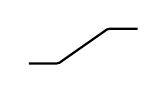
\begin{tikzpicture}[scale=0.22]
                \draw [thick] plot[domain=-pi:pi, samples=40] (\x, {min(1,max(-1, \x*0.7))});
            \end{tikzpicture}
        };

        % Summing junction
        \node [sum, right=1.0cm of sat] (sum1) {};
        \node at ($(sum1.west)+(0.18, 0.08)$)  {\tiny $+$};
        \node at ($(sum1.south)+(0.10, 0.18)$) {\tiny $-$};

        % Gain block
        \node [gainR, right=0.8cm of sum1, label=below:{\small Gain}] (gain) {$\frac{1}{5}$};

        % Integrator block
        \node [block, right=1.0cm of gain, label=below:{\small Integrator}] (int1) {$\dfrac{1}{s}$};

        % To Workspace
        \node [outblock, right=1.2cm of int1, label=below:{\small To Workspace}] (ws) {\small simout};

        % Trigonometric Function block (feedback, below)
        \node [block, below=1.4cm of gain, label=below:{\small Trigonometric\newline Function}] (trig) {\small sin};

        % Tap between int1 and ws
        \coordinate (tap) at ($(int1.east)!0.5!(ws.west)$);
        \filldraw (tap) circle (1.5pt);

        % Forward connections
        \draw [->] (sine)  -- (sat);
        \draw [->] (sat)   -- (sum1);
        \draw [->] (sum1)  -- (gain);
        \draw [->] (gain)  -- (int1);
        \draw [->] (int1)  -- (ws);

        % Feedback: tap -> trig -> sum1.south
        \draw [->] (tap) |- (trig.east);
        \draw [->] (trig.west) -| (sum1.south);

    \end{tikzpicture}
    }
    \caption{Simulink Block Diagram}
\end{figure}

%-----------------------------------
\myproblem{Problem 25}
Use Transfer Function blocks to plot solutions for $0 \le t \le 2$:
\[3\ddot{x} + 15\dot{x} + 18x = f(t),\quad x(0)=\dot{x}(0)=0\]
\[2\ddot{y} + 16\dot{y} + 50y = x(t),\quad y(0)=\dot{y}(0)=0\]
where $f(t) = 75\,u_s(t)$.

\textbf{Problem 25}

Use Transfer Function blocks to plot solutions for $0 \leq t \leq 2$:
\begin{align*}
    3\ddot{x} + 15\dot{x} + 18x &= f(t), \quad x(0) = \dot{x}(0) = 0 \\
    2\ddot{y} + 16\dot{y} + 50y &= x(t), \quad y(0) = \dot{y}(0) = 0
\end{align*}
where $f(t) = 75\,u_s(t)$.

\textbf{Solution:} Taking the Laplace transform with zero initial conditions:
\begin{align*}
    X(s) &= \frac{1}{3s^2+15s+18} \cdot F(s) \\
    Y(s) &= \frac{1}{2s^2+16s+50} \cdot X(s)
\end{align*}
The input $f(t) = 75\,u_s(t)$ is a unit step scaled by 75. Connect a Step block
(amplitude $= 75$) into Transfer Fcn1, whose output feeds Transfer Fcn. Both $x(t)$
and $y(t)$ are collected via a Mux into the \texttt{simout} To~Workspace block.

\begin{figure}[H]
    \centering
    \resizebox{\textwidth}{!}{%
    \begin{tikzpicture}[>=Stealth, node distance=1cm and 1.4cm]
        \tikzset{
            stepblock/.style = {draw, rectangle, minimum height=1.1cm, minimum width=1.1cm, align=center},
            tfblock/.style   = {draw, rectangle, minimum height=1.2cm, minimum width=2.6cm, align=center},
            muxblock/.style  = {draw, rectangle, minimum height=1.4cm, minimum width=0.3cm,
                                align=center, fill=black},
            outblock/.style  = {draw, rectangle, minimum height=1.0cm, minimum width=1.4cm, align=center},
        }

        % Step block (amplitude = 75)
        \node [stepblock, label=below:{\small Step}] (step) {%
            \begin{tikzpicture}[scale=0.25]
                \draw [thick] (-1,-1) -- (-1,0) -- (0,0) -- (0,1) -- (1,1);
                \draw [dashed, thin] (-1,0) -- (1,0);
            \end{tikzpicture}
        };
        \node [below=0.05cm of step, yshift=0.4cm] {\tiny amp $= 75$};

        % Transfer Fcn 1
        \node [tfblock, right=1.2cm of step, label=below:{\small Transfer Fcn1}] (tf1) {%
            $\dfrac{1}{3s^2+15s+18}$
        };

        % Transfer Fcn 2
        \node [tfblock, right=1.4cm of tf1, label=below:{\small Transfer Fcn}] (tf2) {%
            $\dfrac{1}{2s^2+16s+50}$
        };

        % Mux block (solid black bar)
        \node [muxblock, right=1.4cm of tf2] (mux) {};

        % To Workspace
        \node [outblock, right=0.8cm of mux, label=below:{\small To Workspace}] (ws) {\small simout};

        % Tap coordinates
        \coordinate (tapX) at ($(tf1.east)!0.5!(tf2.west)$);
        \coordinate (tapY) at ($(tf2.east)!0.5!(mux.west)$);
        \filldraw (tapX) circle (1.5pt);
        \filldraw (tapY) circle (1.5pt);

        % Forward connections
        \draw [->] (step) -- (tf1);
        \draw [->] (tf1)  -- (tf2);
        \draw [->] (tf2.east) -- (mux.west);
        \draw [->] (mux)  -- (ws);

        % x(t) tap -> mux bottom input
        \draw [->] (tapX) -- ++(0,-1.6) -| (mux.south);

        % Wire labels
        \node [above, font=\small] at (tapX) {$x(t)$};
        \node [above, font=\small] at (tapY) {$y(t)$};

    \end{tikzpicture}
    }
    \caption{Simulink model for Problem 25}
\end{figure}

%-----------------------------------
\myproblem{Problem 28}
Create a Simulink model to plot the solution for $0 \le t \le 1$:
\[\frac{Y(s)}{F(s)} = \frac{4}{s+5}, \qquad f(t) = u_s(t) - u_s(t-1)\]

\begin{figure}[H]
    \centering
    \begin{tikzpicture}[>=Stealth, node distance=1cm and 1.2cm]
        \tikzset{
            stepblock/.style = {draw, rectangle, minimum height=1.1cm, minimum width=1.1cm, align=center},
            tfblock/.style   = {draw, rectangle, minimum height=1.1cm, minimum width=1.8cm, align=center},
            scope/.style     = {draw, rectangle, minimum height=1.1cm, minimum width=1.1cm, align=center},
            sum/.style       = {draw, circle, minimum size=0.8cm, inner sep=0pt},
        }

        % Step blocks with internal step-function shape
        \node [stepblock, label=above left:{\small set start\newline time to 0}] (step1) {%
            \begin{tikzpicture}[scale=0.25]
                \draw [thick] (-1,-1) -- (-1, 0) -- (0, 0) -- (0, 1) -- (1, 1);
                \draw [dashed, thin] (-1, 0) -- (1, 0);
            \end{tikzpicture}
        };

        \node [stepblock, below=1.4cm of step1,
               label=below left:{\small set start\newline time to 1}] (step2) {%
            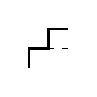
\begin{tikzpicture}[scale=0.25]
                \draw [thick] (-1,-1) -- (-1, 0) -- (0, 0) -- (0, 1) -- (1, 1);
                \draw [dashed, thin] (-1, 0) -- (1, 0);
            \end{tikzpicture}
        };

        % Summing junction (vertically centered between the two step blocks)
        \node [sum, right=1.2cm of step1, yshift=-0.8cm] (sum1) {};
        \node at ($(sum1.west)+(0.18, 0.08)$)  {\tiny $+$};
        \node at ($(sum1.south)+(0.10, 0.18)$) {\tiny $+$};

        % Transfer function block
        \node [tfblock, right=1.0cm of sum1] (tf) {$\dfrac{4}{s+5}$};

        % Scope
        \node [scope, right=1.2cm of tf] (scope) {$\square$};

        % Connections
        \draw [->] (step1.east) -- ++(0.4,0) |- (sum1.west);
        \draw [->] (step2.east) -- ++(0.4,0) |- (sum1.south);
        \draw [->] (sum1) -- (tf);
        \draw [->] (tf)   -- (scope);

    \end{tikzpicture}
    \caption{Simulink Block Diagram}
\end{figure}


%-----------------------------------
\myproblem{Problem 33}
Create a Simulink model for a mass supported by a nonlinear hardening spring, $0 \le t \le 2$:
\[5\ddot{y} = 5g - (900y + 1700y^3), \qquad y(0)=0.5,\;\dot{y}(0)=0\]
Use $g = 9.81$ m/s$^2$.



%-----------------------------------
\myproblem{Problem 35}
The equation for water height $h$ in a spherical tank (radius $r = 3$ m) with drain (radius 2 cm, $C_d = 0.5$), $h(0) = 5$ m:
\[\pi(2rh - h^2)\frac{dh}{dt} = -C_d A\sqrt{2gh}\]
Use Simulink to solve the nonlinear equation and plot $h(t)$ until $h(t) = 0$.

\begin{figure}[H]
    \centering
    \begin{tikzpicture}[>=Stealth, node distance=1cm and 1.2cm]
        \tikzset{
            block/.style   = {draw, rectangle, minimum height=1.0cm, minimum width=1.0cm, align=center},
            outblock/.style= {draw, rectangle, minimum height=0.9cm, minimum width=1.4cm, align=center},
        }

        % Integrator block
        \node [block, label=below:{\small Integrator}] (int1) {$\dfrac{1}{s}$};

        % To Workspace block
        \node [outblock, right=1.2cm of int1, label=below:{\small To Workspace}] (ws) {\small simout};

        % Fcn block (feedback, below)
        \node [block, below=1.2cm of int1, label=below:{\small Fcn}] (fcn) {$f(u)$};

        % Tap coordinate between int1 and ws
        \coordinate (tap) at ($(int1.east)!0.5!(ws.west)$);
        \filldraw (tap) circle (1.5pt);

        % Forward connections
        \draw [->] (int1) -- (ws);

        % Input arrow into integrator
        \draw [->] ($(int1.west)+(-0.8,0)$) -- (int1.west);

        % Feedback: tap -> down -> fcn
        \draw [->] (tap) |- (fcn.east);

        % Fcn output -> back to integrator input
        \draw [->] (fcn.west) -- ++(-0.8,0) |- (int1.west);

    \end{tikzpicture}
    \caption{Simulink Block Diagram}
\end{figure}

%-----------------------------------
\myproblem{Problem 45}
Consider the system in Figure P45 with $m_1=m_2=1$, $c_1=3$, $c_2=1$, $k_1=1$, $k_2=4$:
\[m_1\ddot{x}_1 + (c_1+c_2)\dot{x}_1 + (k_1+k_2)x_1 - c_2\dot{x}_2 - k_2x_2 = 0\]
\[m_2\ddot{x}_2 + c_2\dot{x}_2 + k_2x_2 - c_2\dot{x}_1 - k_2x_1 = f(t)\]
\begin{itemize}
    \item[a.] Develop a Simulink model using state-variable representation.
    \item[b.] Plot $x_1(t)$ for zero initial conditions with piecewise input:
    \[f(t) = \begin{cases} t & 0 \le t \le 1 \\ 2-t & 1 < t < 2 \\ 0 & t \ge 2 \end{cases}\]
\end{itemize}


\begin{figure}[H]
    \centering
    \begin{tikzpicture}[>=Stealth, node distance=1cm and 1.2cm]
        \tikzset{
            rampblock/.style = {draw, rectangle, minimum height=1.1cm, minimum width=1.1cm, align=center},
            ssblock/.style   = {draw, rectangle, minimum height=1.4cm, minimum width=2.0cm, align=center},
            outblock/.style  = {draw, rectangle, minimum height=1.0cm, minimum width=1.4cm, align=center},
            sum/.style       = {draw, circle, minimum size=0.8cm, inner sep=0pt},
        }

        % Ramp blocks with diagonal line inside
        \node [rampblock, label=below:{\small Ramp}]  (ramp0) {%
            \begin{tikzpicture}[scale=0.25]
                \draw [thick] (-1,-1) -- (1,1);
            \end{tikzpicture}
        };
        \node [rampblock, below=0.8cm of ramp0, label=below:{\small Ramp1}] (ramp1) {%
            
\begin{tikzpicture}[scale=0.25]
                \draw [thick] (-1,-1) -- (1,1);
            \end{tikzpicture}
        };
        \node [rampblock, below=0.8cm of ramp1, label=below:{\small Ramp2}] (ramp2) {%
            
\begin{tikzpicture}[scale=0.25]
                \draw [thick] (-1,-1) -- (1,1);
            \end{tikzpicture}
        };

        % Summing junction aligned with ramp1
        \node [sum, right=1.2cm of ramp1] (sum1) {};
        \node at ($(sum1.north)+(0.10,-0.18)$) {\tiny $+$};
        \node at ($(sum1.west)+(0.18, 0.08)$)  {\tiny $+$};
        \node at ($(sum1.south)+(0.10, 0.18)$) {\tiny $+$};

        % State-Space block
        \node [ssblock, right=1.2cm of sum1, label=below:{\small State-Space}] (ss) {%
            \small $x' = Ax+Bu$\\
            \small $y = Cx+Du$
        };

        % To Workspace
        \node [outblock, right=1.2cm of ss, label=below:{\small To Workspace}] (ws) {\small simout};

        % Connections
        \draw [->] (ramp0.east) -- ++(0.4,0) |- (sum1.north);
        \draw [->] (ramp1.east) -- (sum1.west);
        \draw [->] (ramp2.east) -- ++(0.4,0) |- (sum1.south);
        \draw [->] (sum1) -- (ss);
        \draw [->] (ss)   -- (ws);

    \end{tikzpicture}
    \caption{Simulink Block Diagram}
\end{figure}

\vspace{1cm}
\hrule
\vspace{0.5cm}

\end{document}